%=======================================================================
% TCC - Trabalho de Conclusão de Curso (modelo IFC Tradicional 2026)
% Autor: Gabriel Nogueira
% Orientador: Fabricio Bizotto
% Curso: Ciência da Computação - IFC Câmpus Videira
% Ano: 2026
% Codificação: UTF-8 | LaTeX: abnTeX2
%=======================================================================

\documentclass[
	% -- opções da classe memoir --
	12pt,				% tamanho da fonte
	oneside,          % não imprimir em verso e anverso, oposto do twoside
	a4paper,			% tamanho do papel.
	% -- opções da classe abntex2 --
	chapter=TITLE,		% títulos de capítulos convertidos em letras maiúsculas
	section=TITLE,		% títulos de seções convertidos em letras maiúsculas
	subsection=TITLE,	% títulos de subseções convertidos em letras maiúsculas
	%subsubsection=TITLE,% títulos de subsubseções convertidos em letras maiúsculas
	% -- opções do pacote babel --
	english,			% idioma adicional para hifenização
	brazil			% o último idioma é o principal do documento
	,sumario=tradicional,
	]{abntex2-IFC}


% ---
% Pacotes fundamentais 
% ---
\usepackage{cmap}				% Mapear caracteres especiais no PDF
\usepackage{times}			    % Usa a fonte Times
\usepackage[T1]{fontenc}		% Selecao de codigos de fonte.fontenc
\usepackage[utf8]{inputenc}		% Codificacao do documento (conversão automática dos acentos)
\usepackage{lastpage}			% Usado pela Ficha catalográfica
\usepackage{indentfirst}		% Indenta o primeiro parágrafo de cada seção.
\usepackage{color}				% Controle das cores
\usepackage{graphicx}			% Inclusão de gráficos
\usepackage{amsfonts}			% Símbolos
\usepackage{tikz}				% Diagramas (fluxos e arquitetura)
\usetikzlibrary{shapes.geometric, arrows.meta, positioning, fit}
%----Ajuste no alinhamento das listas
\usepackage{enumitem}
\setitemize[0]{itemindent=0.4cm,itemsep=0pt}
\setenumerate[0]{itemindent=0.5cm,itemsep=0pt}
%------
% ---
% Pacotes de citações
% ---
\usepackage[brazilian,hyperpageref]{backref}	 					  % Paginas com as citações na bibl

\usepackage[a4paper]{geometry}
%Referência
\usepackage[alf, 	
			 		abnt-emphasize=bf,
				    abnt-url-package=none,
				    abnt-repeated-title-omit=yes,
				    abnt-full-initials=yes,                                        %yes nome por extenso, no apenas iniciais
					abnt-etal-list=3												%abreviar com mais de 3 autores
]{abntex2/abntex2cite}				 														    % Citações padrão ABNT
\usepackage{lipsum}							   								       % para geração de dummy text
\usepackage{multirow}
\usepackage{float}
\usepackage{setspace}
\usepackage{tabularx}
\usepackage{longtable}

% O \fonte do abnTeX2 sobe 0,5 cm (pensado para figuras em \parbox, como no
% modelo); em tabelas e diagramas TikZ isso sobrepõe a fonte ao conteúdo.
\let\fonteoriginal\fonte
\renewcommand{\fonte}[1]{\par\vspace{0.5cm}\fonteoriginal{#1}}

%\usepackage[none]{hyphenat}
%\captionsetup[table]{justification=raggedright}
% Configurações de aparência do PDF final
% alterando o aspecto da cor azul
\definecolor{blue}{RGB}{41,5,195}

% --- 
% Espaçamentos entre linhas e parágrafos 
% --- 
% O tamanho do parágrafo é dado por:
\setlength{\parindent}{2cm}
\linespread{1.5}

%Espaçamento depois dos títulos
\setlength{\afterchapskip}{\baselineskip}
% %\setlength{\afterchapskip}{\lineskip}

% Controle do espaçamento entre um parágrafo e outro:
\setlength{\parskip}{0cm}  % tente também \onelineskip

\hangcaption
\captionstyle[\raggedright]{}

%Estava mostrando nas referencias quais paginas estavam sendo referenciadas
\renewcommand{\backref}{}
\renewcommand*{\backrefalt}[4]{}

%Reduzir a fonte do caption
%\captionnamefont{\centering\ABNTEXfontereduzida}
%\captiontitlefont{\centering\ABNTEXfontereduzida}
%Ajuste nas listas de tabela, ilustrações e quadros
\setlength\cftbeforechapterskip{0pt}
% ---
% compila o indice
% ---
\makeindex
% ---

%----Include da capa é fora do documento
% ---
% Informações de dados para CAPA e FOLHA DE ROSTO
% ---

\titulo{\uppercase{Classificação Fiscal NCM Assistida por Modelos de Linguagem Executados Localmente, com Supervisão Humana, em um Sistema ERP}}
\autor{\uppercase{Gabriel Nogueira}}
\local{Videira}
\data{2026}
\orientador[Orientador:]{Fabricio Bizotto}
\instituicao{ Ministério da Educação\\
        Secretaria de Educação Profissional e Tecnológica\\
        Instituto Federal Catarinense\\
        Câmpus Videira}
\tipotrabalho{Trabalho de Conclusão de Curso}
% O preambulo deve conter o tipo do trabalho, o objetivo,
% o nome da instituição e a área de concentração
\preambulo{Trabalho de Conclusão de Curso apresentado ao
Curso de graduação em Ciência da Computação do
Instituto Federal Catarinense – Câmpus Videira para
obtenção do título de bacharel em Ciência da Computação.

Orientador: \imprimirorientador}
% ---

%---

\begin{document}
% Retira espaço extra obsoleto entre as frases.
\frenchspacing

% ----------------------------------------------------------
% ELEMENTOS PRÉ-TEXTUAIS
% ----------------------------------------------------------

%--- CAPA ----
\imprimircapa

% --- FOLHA DE ROSTO
\imprimirfolhaderosto
% \imprimirfolhaderosto* (o * indica que haverá a ficha bibliográfica)

% Inserir FOLHA DE APROVAÇÃO
\begin{folhadeaprovacao}

  \begin{center}
  \vspace*{-1.2cm}
    \textbf{\large\imprimirautor}
    
    \vspace*{\fill}\vspace*{\fill}\vspace*{\fill}
    \parbox{15cm}{
        \OnehalfSpacing\centering\large\textbf{\imprimirtitulo}
    }
    \vspace*{\fill}\vspace*{\fill}
    
    \hspace{.45\textwidth}
    \begin{minipage}{.5\textwidth}
        Este Trabalho de Curso foi julgado
        adequado para a obtenção do título de
        Bacharel em Ciência da Computação e
        aprovado em sua forma final pelo curso de
        graduação em Ciência da Computação do Instituto Federal Catarinense
        – Campus Videira. 

    \end{minipage}%
    \vspace*{\fill}
   \end{center}
    \vspace{-1cm}
  \begin{center}
  	 Videira (SC), dia de mês de ano
  \end{center}
  

    %\vspace{-1cm}

  
   \assinatura{\begin{center}\vspace{-0.7cm}\imprimirorientador \\ 
   					   Instituto Federal Catarinense – Campus Videira
   					   \end{center}
   			  } 
    \begin{center}
  	\textbf{ BANCA EXAMINADORA}
   \end{center}
   %\vspace{-1cm}
   \assinatura{\begin{center}\vspace{-0.7cm}Fabio Pinheiro\\
   					   Instituto Federal Catarinense – Campus Videira
   					     \end{center}
   }
    \assinatura{\begin{center}\vspace{-0.7cm}Tiago Heineck \\
   					    Instituto Federal Catarinense – Campus Videira
   					    \end{center}
    }
    

    \vspace*{1cm}
  
\end{folhadeaprovacao}

% Inserir FOLHA DE AUTORIZAÇÃO (versão final, após a defesa)
% \begin{folhadeautorizacao}

  \begin{center}
  \vspace*{1 cm}
  \vspace{-2cm}
   \centering
\includegraphics[width=1.5cm]{brasaoRepublicaPeB.jpg}
   \vspace{-0.5 cm}
    {\large \SingleSpacing \imprimirinstituicao}
    \vspace{-0.5cm}
    \center{ \hrulefill}
    
     {\large \SingleSpacing \textbf{Autorização}}
    
    
    \vspace*{1 cm}
    
    \raggedleft{ Videira (SC), 19 de Novembro de 2016}
    \vspace*{0.5 cm}
    
   \end{center}
   


Eu, NOME SOBRENOME, regularmente matriculado na disciplina de Trabalho de Conclusão de Curso II - TC II do curso de Bacharel em Ciência da Computação, sob matrícula nº. XXXXXXX, pelo presente documento, autorizo o Instituto Federal Catarinense - IFC-Câmpus Videira, a utilizar o meu TC II intitulado "\imprimirtitulo", sob a orientação d Professor \imprimirorientador, para futuras informações e divulgações promovidas pelo Curso, e pelo Instituto, de forma institucional, em todo território nacional e internacional, sem fins comerciais, por qualquer meio de comunicação, tornando-o acessível a qualquer pessoa com interesse no trabalho.

A presente autorização substancia um consentimento de vontade e isenta de qualquer vício, feito de forma gratuita, e no gozo da minha capacidade civil, pelo que declaro nada me ser devido pelo curso de Ciência da Computação e pelo IFC-Câmpus Videira, ou seus representantes, em tempo algum, seja que título for, no que se refere, direta ou indiretamente, ao presente consentimento de uso da minha imagem e meu trabalho.

Declaro, ainda, que a utilização de meu nome e de meu trabalho, não constitui ofensa ou violação de meus direitos, nos termos do inciso X, do artigo 5o. da Constituição Federal.

Pelo presente também declaro ser de minha total responsabilidade o conteúdo de meu trabalho de conclusão de curso, descrito neste documento.

Os direitos e as obrigações aqui avençados transmitem-se aos meus herdeiros e sucessores.



  
   
   \vspace*{\fill}
   \vspace{-0.5 cm}
   
   \noindent Nome: \imprimirautor
   
   \vspace{0.25 cm}
   
   \noindent CPF: XXXXXXXXXXXXXX
   
   \vspace{0.25 cm}
   
   \noindent Assinatura: \hskip-3em\vtop{\vskip.05cm\hsize=5in \hrulefill}
   
   \vspace{0.5 cm}
   
    \begin{center}
    Rod. SC 135, KM 125 - Campo Experimental - CEP: 89560-000 - Videira - SC \\
    Fone: (49) 3533-4900 - http://www.ifc-videira.edu.br
    \end{center}

    \vspace*{1cm}
  
\end{folhadeautorizacao}

% DEDICATÓRIA, AGRADECIMENTOS e EPÍGRAFE (opcionais) -- ativar na versão final
% \begin{dedicatoria}
 \vspace*{\fill}
 \noindent
  \raggedleft
 \begin{minipage}{.54\textwidth}
    Dedico este trabalho ...
   \end{minipage}
\end{dedicatoria}

% \begin{agradecimentos}

agradecimentos

\end{agradecimentos}

% RESUMO E ABSTRACT
% ---
% resumo em português
\begin{resumo}
\noindent
Inconsistências na classificação fiscal de produtos em sistemas de gestão empresarial (ERPs), como a Nomenclatura Comum do Mercosul (NCM) vazia, inexistente ou de outro produto, levam à rejeição da Nota Fiscal Eletrônica ou à tributação incorreta e geram demanda recorrente ao suporte técnico. Este trabalho desenvolve e avalia um protótipo de classificação fiscal NCM assistida por Modelos de Linguagem de Grande Escala (LLMs) executados localmente, integrado ao banco de dados Firebird do ERP Lux Auto, no qual o modelo apenas sugere e nenhuma alteração é gravada sem aprovação humana. Códigos inválidos são detectados por consulta determinística à tabela oficial. A sugestão combina a expansão de abreviações, uma busca lexical (SQLite FTS5 com BM25, sinônimos e fusão de rankings), uma base de conhecimento com produtos já classificados por duas lojas de autopeças, consultada por vizinhos mais próximos, e duas escolhas do modelo Qwen3 8B restritas por esquema JSON, de modo que o modelo só pode responder com códigos existentes. Códigos válidos são apontados como possivelmente incorretos quando ficam fora das três sugestões e o modelo julga o texto oficial incompatível com o produto. A avaliação usou conjuntos separados de desenvolvimento e de teste, este medido uma única vez. A detecção apontou todos os códigos vazios, malformados, inexistentes e extintos, sem falsos positivos em mais de 41 mil produtos reais; para códigos válidos, porém incorretos, teve acurácia de 86,6\% no desenvolvimento e de 88,8\% em erros reais de uma loja, em que apontou todos os 40 produtos cadastrados com um código ``coringa'', e de 86,0\% no teste, com 6,0\% de alarmes falsos. Na sugestão, a versão final acertou o código em primeiro lugar em 48,0\% e entre as três opções em 58,0\% dos 50 produtos de teste, em 13,7 segundos por produto, contra 20,0\% e 30,0\% da busca sem modelo de linguagem; nos produtos automotivos, foco do ERP, acertou 83,3\% em primeiro lugar. A meta de 75\% de acerto foi atingida apenas no recorte automotivo, e a maior parte dos erros restantes decorre da distância entre o nome comercial do produto e o texto oficial da tabela. Os resultados indicam que um LLM pequeno executado localmente é viável como assistente de classificação fiscal, desde que restrito a escolher entre candidatos verificados, apoiado em exemplos reais e subordinado à aprovação humana.

\vspace{\onelineskip}
\noindent
\textbf{Palavras-chave}: Modelos de Linguagem de Grande Escala. Classificação Fiscal. NCM. Geração Aumentada por Recuperação. \textit{Human-in-the-Loop}. ERP.
\end{resumo}

% resumo em inglês
\begin{resumo}[Abstract]
\begin{otherlanguage*}{english}
\noindent
Inconsistencies in the tax classification of products in Enterprise Resource Planning (ERP) systems, such as a Mercosur Common Nomenclature (NCM) code that is empty, nonexistent or belongs to another product, cause Brazilian electronic invoices to be rejected or taxed incorrectly and create recurring demand for technical support. This work develops and evaluates a prototype for NCM classification assisted by locally run Large Language Models (LLMs), integrated with the Firebird database of the Lux Auto ERP, in which the model only suggests and no change is written without human approval. Invalid codes are detected by a deterministic lookup in the official table. Suggestion combines abbreviation expansion, lexical retrieval (SQLite FTS5 with BM25, synonyms and rank fusion), a knowledge base of products already classified by two auto parts stores, queried by nearest neighbors, and two choices by the Qwen3 8B model constrained by a JSON schema, so the model can only answer with existing codes. Valid codes are flagged as possibly incorrect when they fall outside the three suggestions and the model judges the official text incompatible with the product. The evaluation used separate development and test sets, the latter measured only once. Detection flagged every empty, malformed, nonexistent and discontinued code, with no false positives among more than 41 thousand real products; for valid but incorrect codes, it reached 86.6\% accuracy in development and 88.8\% on real errors from one store, where it flagged all 40 products registered with a ``catch-all'' code, and 86.0\% on the test set, with a 6.0\% false alarm rate. For suggestion, the final version ranked the correct code first for 48.0\% and among the three options for 58.0\% of the 50 test products, in 13.7 seconds per product, against 20.0\% and 30.0\% for retrieval without a language model; for automotive products, the focus of the ERP, it ranked the correct code first for 83.3\%. The 75\% accuracy target was met only for automotive products, and most remaining errors come from the gap between commercial product names and the official table text. The results indicate that a small, locally run LLM is viable as a tax classification assistant, provided it is restricted to choosing among verified candidates, supported by real examples and subordinate to human approval.

\vspace{\onelineskip}
\noindent
\textbf{Keywords}: Large Language Models. Tax Classification. NCM. Retrieval-Augmented Generation. Human-in-the-Loop. ERP.
\end{otherlanguage*}
\end{resumo}


% LISTA DE ILUSTRAÇÕES
\pdfbookmark[0]{\listfigurename}{lof}
\listoffigures*
\cleardoublepage

% LISTA DE QUADROS
\pdfbookmark[0]{\listofquadrosname}{loq}
\listofquadros*
\cleardoublepage

% LISTA DE TABELAS
\pdfbookmark[0]{\listtablename}{lot}
\listoftables*
\cleardoublepage

% LISTA DE ABREVIATURAS E SIGLAS
\begin{siglas}
  \item[API] \textit{Application Programming Interface}
  \item[BM25] \textit{Best Matching 25} (função de ranqueamento)
  \item[CBS] Contribuição sobre Bens e Serviços
  \item[CFOP] Código Fiscal de Operações e Prestações
  \item[CST] Código de Situação Tributária
  \item[ERP] \textit{Enterprise Resource Planning}
  \item[FTS] \textit{Full-Text Search}
  \item[GECEX] Comitê Executivo de Gestão da Câmara de Comércio Exterior
  \item[GPU] \textit{Graphics Processing Unit}
  \item[HITL] \textit{Human-in-the-Loop}
  \item[HTS] \textit{Harmonized Tariff Schedule}
  \item[IBS] Imposto sobre Bens e Serviços
  \item[ICMS] Imposto sobre Circulação de Mercadorias e Serviços
  \item[JSON] \textit{JavaScript Object Notation}
  \item[kNN] \textit{k-Nearest Neighbors} (vizinhos mais próximos)
  \item[LGPD] Lei Geral de Proteção de Dados Pessoais
  \item[LLM] \textit{Large Language Model}
  \item[MOC] Manual de Orientação do Contribuinte
  \item[NBS] Nomenclatura Brasileira de Serviços
  \item[NCM] Nomenclatura Comum do Mercosul
  \item[NF-e] Nota Fiscal Eletrônica
  \item[RAG] \textit{Retrieval-Augmented Generation}
  \item[RGI] Regras Gerais de Interpretação do Sistema Harmonizado
  \item[RRF] \textit{Reciprocal Rank Fusion}
  \item[SEFAZ] Secretaria da Fazenda
  \item[SH] Sistema Harmonizado de Designação e de Codificação de Mercadorias
  \item[SQL] \textit{Structured Query Language}
  \item[SVM] \textit{Support Vector Machine}
  \item[TEC] Tarifa Externa Comum
  \item[VRAM] \textit{Video Random Access Memory}
\end{siglas}


% SUMARIO
\pdfbookmark[0]{\contentsname}{toc}
\tableofcontents*
\cleardoublepage

% ------------------------------------------------------
% ELEMENTOS TEXTUAIS
% ------------------------------------------------------
\textual

\chapter{INTRODUÇÃO}

Nos dias atuais, sistemas de gestão empresarial (ERPs) dependem fortemente da inserção manual de dados cadastrais para o seu pleno funcionamento. Essa dependência operacional gera gargalos significativos, uma vez que a interação humana está sujeita a falhas de digitação ou interpretação \cite{Mehta2025ERPDataQuality}. Tais inconsistências em bancos de dados relacionais dividem-se, em geral, em duas categorias. A primeira envolve erros de preenchimento que não impedem o funcionamento básico do sistema, como a inserção de um número de telefone no campo destinado ao endereço. A segunda, e mais crítica, engloba informações que afetam diretamente o ecossistema de integrações do software. Um exemplo claro ocorre no módulo fiscal: quando o cadastro de um cliente apresenta divergências entre a Inscrição Estadual e o Indicador de Contribuinte, ou há a omissão e preenchimento incorreto de códigos obrigatórios como NCM (Nomenclatura Comum do Mercosul), CST (Código de Situação Tributária) e CFOP (Código Fiscal de Operações e Prestações), a emissão da Nota Fiscal Eletrônica (NF-e) é inviabilizada e sumariamente rejeitada pela Secretaria da Fazenda (SEFAZ) \cite{brasil2020moc}.

Essas rejeições paralisam o faturamento das empresas e geram uma sobrecarga imediata no setor de suporte técnico, exigindo intervenção manual para correções que, na maioria das vezes, seguem padrões lógicos e regulatórios bem definidos. Nesse cenário, os Modelos de Linguagem de Grande Escala (LLMs) surgem como uma alternativa tecnológica promissora \cite{Wang2023LLMAgentsSurvey}. Combinados a regras de negócio predefinidas, eles podem ajudar a identificar anomalias e a formular propostas de correção \cite{Roychowdhury2025NLIDB}. Para garantir a segurança e a integridade da operação no banco de dados, o modelo não age de forma autônoma: ele apenas sugere, e a correção proposta aguarda a validação e a aprovação de um operador humano antes de ser executada, no paradigma conhecido como \textit{Human-in-the-Loop} \cite{Cheng2026DecoupledHITL}.

Dentre as inconsistências fiscais, a classificação do produto pela NCM se destaca por exigir interpretação. Verificar se um código existe é uma consulta simples; descobrir qual código corresponde a uma descrição como ``PARACHOQUE DIANTEIRO GOL'' ou ``AZULEJO DE BANHEIRO'' exige conhecer uma tabela com mais de dez mil itens, organizada hierarquicamente e redigida em linguagem técnica que raramente coincide com o nome comercial do produto \cite{receita2026ncm}. Além disso, um código pode existir na tabela e, ainda assim, pertencer a outro produto, erro que nenhuma consulta simples detecta. Por esses motivos, este trabalho concentra a implementação e a avaliação na NCM do cadastro de produtos, deixando as demais categorias delimitadas no projeto (CST, CFOP e Indicador de Contribuinte) como continuidade natural da arquitetura proposta.

Diante deste contexto, o presente trabalho busca responder à seguinte pergunta de pesquisa: em que medida um modelo de linguagem de pequeno porte, executado localmente e restrito a escolher entre candidatos recuperados da tabela oficial, consegue apontar classificações NCM inválidas ou incorretas no cadastro de produtos de um ERP e sugerir a classificação correta, em tempo compatível com o uso diário e sob supervisão humana?

\section{Objetivos}

\subsection{Objetivo Geral}

Desenvolver e avaliar um protótipo de classificação fiscal NCM assistida por modelos de linguagem executados localmente, integrado ao banco de dados do ERP Lux Auto, que aponte produtos com NCM inválido ou possivelmente incorreto e sugira a classificação a partir da descrição do produto, com aprovação humana obrigatória antes de qualquer alteração no banco de dados.

\subsection{Objetivos Específicos}

\begin{itemize}
    \item Delimitar, a partir da experiência do autor no suporte técnico do Lux Auto, as inconsistências fiscais do cadastro que impedem a emissão de NF-e, e justificar a escolha da classificação NCM de produtos como foco da implementação;
    \item Estruturar a tabela NCM oficial em uma base local consultável, que permita validar códigos e recuperar candidatos a partir de descrições livres sem enviar a tabela inteira ao modelo de linguagem;
    \item Projetar e implementar o protótipo, com detecção de NCM inválido, detecção de NCM possivelmente incorreto, sugestão de classificação, execução em segundo plano e aprovação por meio de uma interface independente do ERP;
    \item Construir conjuntos de avaliação separados para desenvolvimento e para teste, com a classificação correta de cada produto conferida na tabela oficial, incluindo códigos inválidos de diferentes tipos e erros de classificação reais extraídos de bases de clientes;
    \item Avaliar o protótipo quanto à detecção, ao acerto das sugestões e ao tempo de resposta, medindo a contribuição do modelo de linguagem em relação à busca sem modelo e comparando modelos abertos e arquiteturas alternativas.
\end{itemize}

\section{Justificativa}

A gestão fiscal em sistemas ERP representa um dos principais gargalos operacionais em pequenas e médias empresas do setor automotivo. Inconsistências cadastrais, como divergências entre a Inscrição Estadual e o Indicador de Contribuinte e o preenchimento incorreto de códigos NCM, CST e CFOP, comprometem diretamente a emissão de NF-e, interrompendo o fluxo de faturamento. Problemas de qualidade de dados são reconhecidos como fonte recorrente de dificuldades na operação de ERPs \cite{xu2002}, e, na experiência do autor no suporte técnico do Lux Auto, erros cadastrais de natureza fiscal estão entre os motivos recorrentes de chamados abertos pelos clientes. Essa observação não se apoia em um levantamento quantitativo do sistema de chamados, que não foi realizado neste trabalho, mas na prática diária de atendimento; por isso, ela é apresentada como delimitação do problema, e não como medida de sua frequência. A Figura~\ref{fig:fluxo_rejeicao} sintetiza o fluxo que origina essa demanda.

\begin{figure}[H]
    \centering
    \caption{Fluxo de rejeição de NF-e e geração de demanda de suporte técnico}
    \label{fig:fluxo_rejeicao}
    \begin{tikzpicture}[
        node distance=1.2cm,
        every node/.style={font=\small},
        box/.style={rectangle, draw, rounded corners=4pt, minimum width=5.2cm, minimum height=0.9cm, align=center, fill=blue!8, text width=5cm},
        errorbox/.style={rectangle, draw, rounded corners=4pt, minimum width=5.2cm, minimum height=0.9cm, align=center, fill=red!10, text width=5cm},
        arrow/.style={-{Stealth[scale=1]}, thick}
    ]
        \node (cadastro)  [box]      {Operador preenche cadastro\\com dado incorreto};
        \node (emissao)   [box,      below=of cadastro] {Sistema ERP tenta\\emitir a NF-e};
        \node (sefaz)     [errorbox, below=of emissao]  {SEFAZ rejeita o documento\\(código de erro técnico)};
        \node (suporte)   [errorbox, below=of sefaz]    {Abertura de chamado ao\\suporte técnico};

        \draw [arrow] (cadastro) -- (emissao);
        \draw [arrow] (emissao)  -- (sefaz);
        \draw [arrow] (sefaz)    -- node[right, font=\footnotesize] {erro não compreendido pelo operador} (suporte);
    \end{tikzpicture}
    \fonte{O autor (2026).}
\end{figure}

Embora os próprios sistemas ERP sinalizem esses erros ao usuário, a baixa familiaridade dos operadores com terminologia fiscal faz com que as mensagens de erro sejam frequentemente ignoradas, resultando em chamados de suporte para problemas que já foram identificados pelo sistema, mas não compreendidos pelo usuário. Esse comportamento evidencia que a solução não passa apenas por detectar o erro, mas por interpretá-lo e propor uma correção acessível e supervisionada, de preferência no momento do cadastro, antes que a nota seja emitida.

Nesse contexto, regras fixas resolvem apenas parte do problema. Uma regra consegue dizer que o NCM ``00000000'' é inválido, mas não consegue dizer que um ``PARACHOQUE'' deve ser classificado em ``8708.10.00 -- Para-choques e suas partes'': isso exige interpretar a descrição do produto e relacioná-la ao texto da tabela oficial, tarefa em que os LLMs têm demonstrado bom desempenho \cite{gholamian2024llmclassification}. Ao mesmo tempo, o risco de alucinação desses modelos \cite{huang2025hallucination} torna indispensável que a resposta seja verificável e que a decisão final permaneça com um humano \cite{Natarajan2024AI2L}. Investigar como equilibrar essas duas necessidades com um modelo pequeno, executado localmente e sem custo de API, e medir quanto o modelo de linguagem acrescenta em relação a uma busca sem ele, é a contribuição prática deste trabalho.

\section{Estrutura do Trabalho}

O Capítulo~\ref{cap:fundamentacao} apresenta a fundamentação teórica: sistemas ERP e qualidade de dados, a NF-e e a estrutura da NCM, os LLMs e a engenharia de \textit{prompt}, as técnicas de recuperação de informação e de avaliação empregadas e os trabalhos correlatos, incluindo estudos de classificação automática de NCM e do SH. O Capítulo~\ref{cap:metodologia} descreve a metodologia, incluindo o ambiente experimental, os conjuntos de casos e as métricas. O Capítulo~\ref{cap:desenvolvimento} detalha a arquitetura e a implementação do protótipo, bem como as versões testadas e descartadas ao longo do desenvolvimento. O Capítulo~\ref{cap:resultados} apresenta e discute os resultados, e o Capítulo~\ref{cap:conclusao} traz as conclusões e os trabalhos futuros.

\chapter{FUNDAMENTAÇÃO TEÓRICA}
\label{cap:fundamentacao}

Neste capítulo, são apresentados os conceitos e tecnologias que embasam o desenvolvimento deste trabalho. São abordados o funcionamento dos sistemas ERP e os desafios de qualidade de dados, as exigências da legislação fiscal brasileira para emissão de Notas Fiscais Eletrônicas e a estrutura da NCM, os fundamentos dos Modelos de Linguagem de Grande Escala e da engenharia de \textit{prompt}, a abordagem de agentes com supervisão humana, as técnicas de recuperação de informação empregadas, os conceitos de avaliação experimental adotados, a integração de LLMs com bancos de dados relacionais, apresentada como contraste com a abordagem deste trabalho, e, por fim, os trabalhos correlatos, com ênfase na classificação automática de NCM e do Sistema Harmonizado.

\section{Sistemas ERP}

Os sistemas de gestão empresarial, conhecidos pela sigla ERP (do inglês \textit{Enterprise Resource Planning}), são plataformas de software integradas que centralizam e automatizam os principais processos organizacionais em um único ambiente \cite{arora2017}. Esses sistemas abrangem módulos como financeiro, fiscal, controle de estoque, vendas e relacionamento com clientes, permitindo que informações fluam entre os departamentos de forma padronizada. Sua adoção por pequenas e médias empresas tem crescido de forma expressiva nas últimas décadas, impulsionada pela necessidade de maior controle operacional e pela exigência de conformidade com normas regulatórias cada vez mais rigorosas \cite{laukkanen2007erp,vanEverdingen2000erp}.

No setor automotivo brasileiro, especificamente em oficinas mecânicas, os sistemas ERP assumem papel estratégico. Dados do Anuário da Indústria de Reparação de Veículos indicam que o Brasil possui mais de 119 mil estabelecimentos do ramo automotivo \cite{sindirepa2023}, o que evidencia a dimensão do mercado e a necessidade de eficiência operacional nesses negócios. Nesse contexto, o ERP integra o controle de ordens de serviço, a gestão de peças e insumos, o cadastro de clientes e fornecedores e a emissão de documentos fiscais em um único fluxo, tornando a consistência dos dados cadastrais um requisito não apenas técnico, mas legal.

Um exemplo prático dessa realidade é o sistema ERP Lux Auto, voltado ao segmento de oficinas mecânicas, desenvolvido em Delphi e com banco de dados Firebird. O sistema contempla o registro de produtos, o controle de serviços prestados em veículos, cadastros gerais de pessoas e fornecedores, além de módulos de contas a receber e a pagar. Embora ofereça uma interface funcional para usuários experientes, na experiência do autor no suporte técnico, novos clientes frequentemente enfrentam dificuldades nos primeiros meses de uso, e é no módulo fiscal que os problemas mais críticos surgem, pois as validações impostas pelos órgãos governamentais são rígidas e intolerantes a erros de formatação ou classificação.

\subsection{Qualidade de Dados em Sistemas ERP}

A qualidade dos dados armazenados em sistemas ERP é fator determinante para a confiabilidade dos processos organizacionais \cite{xu2002}. Inconsistências cadastrais, sejam elas provenientes de erros de digitação, falta de padronização ou desconhecimento técnico dos operadores, comprometem a integridade das informações e geram um efeito cascata em todos os processos dependentes desses dados \cite{krishna2024}. No contexto fiscal, essas inconsistências assumem caráter crítico: campos como Inscrição Estadual, Indicador de Contribuinte, NCM, CST e CFOP são validados por órgãos reguladores no momento da emissão de documentos fiscais eletrônicos \cite{brasil2020moc}. A presença de dados incorretos ou em branco nesses campos inviabiliza o faturamento da empresa emissora, gerando demanda urgente e recorrente ao suporte técnico \cite{Mehta2025ERPDataQuality}.

Os ERPs atendem negócios dos mais variados perfis, e no nicho de oficinas mecânicas essa discrepância de conhecimento tecnológico fica ainda mais evidente. O sistema precisa atender desde profissionais qualificados em rotinas fiscais até usuários com pouca familiaridade com computação básica. Na experiência do autor com o Lux Auto, a maioria dos gargalos operacionais recai sobre usuários que não conseguem, por conta própria, ajustar campos como NCM ou Indicador de Contribuinte a partir de um código de rejeição devolvido pela SEFAZ. Nesse cenário, mecanismos de validação e correção preventiva, que atuem no momento do cadastro, tornam-se essenciais para manter a operação do negócio ativa \cite{Schelter2018DQVerify}.

\section{Nota Fiscal Eletrônica e Legislação Fiscal Brasileira}

A Nota Fiscal Eletrônica (NF-e) é um documento fiscal digital instituído pelo Ajuste SINIEF 07/2005, que substituiu o modelo em papel e conferiu maior agilidade e controle às operações comerciais \cite{sinief2005}. Sua emissão é regulamentada pela SEFAZ e está condicionada à validação em tempo real por meio de serviços web governamentais, que verificam centenas de regras de negócio antes de autorizar o documento \cite{brasil2020moc}.

Entre os principais campos obrigatórios validados pela SEFAZ, destacam-se o Código de Situação Tributária (CST), que define o tratamento do ICMS aplicável à operação; o Código Fiscal de Operações e Prestações (CFOP), que classifica a natureza da operação comercial; e a Nomenclatura Comum do Mercosul (NCM), que identifica a classificação fiscal do produto e determina suas alíquotas tributárias \cite{sefazpe2016}. Além desses, o documento exige a descrição detalhada dos produtos, tributos como IPI, PIS, COFINS e ISS e os dados completos do emitente e do destinatário \cite{brasil2020moc}. O Manual de Orientação do Contribuinte define essas validações e associa a cada uma delas um código de rejeição: basta que uma regra não seja atendida, por exemplo um código NCM inexistente na tabela vigente, para que o documento seja rejeitado, interrompendo o fluxo de faturamento da empresa emissora \cite{brasil2020moc}.

Com a reforma tributária em curso no Brasil \cite{brasil2023ec132}, que substitui progressivamente os tributos vigentes pelo IBS (Imposto sobre Bens e Serviços) e pela CBS (Contribuição sobre Bens e Serviços), os documentos fiscais eletrônicos passam a exigir novos campos e regras de classificação durante o período de transição. Para sistemas ERP, isso amplia o espaço de possíveis inconsistências cadastrais, tornando ainda mais improvável que um sistema baseado apenas em regras fixas acompanhe todas as combinações válidas. Abordagens que combinam LLMs com representações formais das regras tributárias têm sido propostas como forma de manter a confiabilidade do raciocínio fiscal diante de mudanças regulatórias frequentes \cite{Jurayj2025TaxLogic}.

\subsection{Nomenclatura Comum do Mercosul}
\label{sec:ncm}

A NCM é o sistema de classificação de mercadorias adotado pelos países do Mercosul, utilizado tanto no comércio exterior quanto nas operações internas, como a emissão de NF-e \cite{receita2026ncm}. Ela tem por base o Sistema Harmonizado de Designação e de Codificação de Mercadorias (SH), mantido pela Organização Mundial das Aduanas, que padroniza internacionalmente os seis primeiros dígitos do código \cite{wco2026hs}. A NCM acrescenta dois dígitos próprios, formando um código de oito dígitos organizado de forma hierárquica, como ilustra a Figura~\ref{fig:hierarquia_ncm}: os dois primeiros identificam o Capítulo; os quatro primeiros, a Posição; o quinto e o sexto, as Subposições; e o sétimo e o oitavo, o Item e o Subitem. Somente o código completo de oito dígitos é válido para o cadastro de um produto.

\begin{figure}[H]
    \centering
    \caption{Estrutura hierárquica de um código NCM}
    \label{fig:hierarquia_ncm}
    \begin{tikzpicture}[
        node distance=0.45cm,
        every node/.style={font=\small},
        nivel/.style={rectangle, draw, rounded corners=3pt, align=left, fill=blue!8, text width=12.5cm, minimum height=0.8cm},
        folha/.style={rectangle, draw, rounded corners=3pt, align=left, fill=green!10, text width=12.5cm, minimum height=0.8cm}
    ]
        \node (cap)  [nivel] {\textbf{87} \quad Capítulo: Veículos automóveis, tratores, ciclos e outros veículos terrestres, suas partes e acessórios};
        \node (pos)  [nivel, below=of cap] {\textbf{87.08} \quad Posição: Partes e acessórios dos veículos automóveis das posições 87.01 a 87.05};
        \node (item) [folha, below=of pos] {\textbf{8708.10.00} \quad Item: Para-choques e suas partes \hfill (único nível válido no cadastro)};
    \end{tikzpicture}
    \fonte{O autor (2026), com base na Tabela NCM vigente.}
\end{figure}

A tabela vigente utilizada neste trabalho possui 96 capítulos e 10.504 códigos de oito dígitos. Duas características dessa tabela são centrais para o problema estudado. A primeira é que a descrição própria de um item frequentemente só faz sentido junto com os níveis superiores: o item 4011.10.00 é descrito apenas como ``Do tipo utilizado em automóveis de passageiros'', e é o cabeçalho da posição 40.11 que informa tratar-se de pneumáticos novos de borracha. A segunda é que o texto oficial usa linguagem técnica, distante do nome comercial do produto: ``sabonete'' aparece como ``sabões'', ``cadeira'' como ``assentos'' e ``notebook'' como ``máquinas automáticas para processamento de dados''. Além disso, a classificação segue as Regras Gerais de Interpretação do Sistema Harmonizado (RGI), que integram o texto da Convenção do SH, promulgada no Brasil pelo Decreto nº 97.409/1988 \cite{brasil1988sh}, e são reproduzidas na NCM vigente, aprovada pela Resolução Gecex nº 272/2021 \cite{gecex2021}. Pela primeira regra, os títulos das seções e dos capítulos têm valor apenas indicativo, e a classificação é determinada pelos textos das posições e das notas de seção e de capítulo; pela sexta, a mesma lógica se aplica, dentro de uma posição, às subposições. As notas são, portanto, parte da classificação: a Nota 2 da Seção XVII, por exemplo, exclui das ``partes e acessórios'' de veículos as peças de uso geral, como parafusos, rolamentos e artigos de borracha, que têm posição própria mesmo quando destinadas a automóveis \cite{gecex2021}.

A tabela também muda ao longo do tempo. A cada atualização, códigos são criados e outros são extintos, e um produto cadastrado com um código extinto passa a ter a nota rejeitada, ainda que o código tenha sido válido quando foi informado. Na atualização em vigor a partir de 1º de setembro de 2022, por exemplo, o código 3923.30.00 foi substituído por 3923.90.10 e 3923.90.90, e o 9403.20.00, por 9403.20.10 e 9403.20.90 \cite{encat2022nt}.

Cabe observar que, no Lux Auto, o mesmo campo do cadastro guarda também códigos de serviços, que seguem outra classificação, a Nomenclatura Brasileira de Serviços (NBS). Por isso, a validação da NCM deve se restringir aos itens cadastrados como mercadoria, sob pena de apontar como erro um código de serviço legítimo.

\section{Modelos de Linguagem de Grande Escala}

Os Modelos de Linguagem de Grande Escala, conhecidos pela sigla LLM (do inglês \textit{Large Language Model}), são sistemas de inteligência artificial baseados na arquitetura \textit{Transformer}, proposta por \citeonline{vaswani2017attention}. Essa arquitetura utiliza mecanismos de autoatenção (\textit{self-attention}) que permitem ao modelo processar sequências de texto de forma paralela, identificando relações contextuais entre palavras independentemente de sua posição na sentença \cite{shao2024}. Os LLMs são treinados em volumes massivos de dados textuais, o que lhes confere a capacidade não apenas de gerar texto coerente, mas de interpretar contextos complexos e inferir intenções \cite{douglas2023}.

No domínio tributário, essa capacidade tem sido investigada com resultados promissores, mas ainda limitados. Em um estudo sobre a aplicação do direito tributário dos Estados Unidos, \citeonline{Nay2023TaxAttorneys} observaram que o desempenho dos LLMs melhora a cada nova geração de modelos e, sobretudo, quando o modelo recebe os textos legais pertinentes e exemplos de perguntas e respostas junto com a pergunta, embora ainda sem atingir o nível de especialistas. Embora trate de outra legislação, o resultado indica dois recursos explorados neste trabalho: fornecer ao modelo o texto oficial relevante e orientá-lo com exemplos. A classificação de um produto pelo código NCM, por exemplo, exige a interpretação de descrições textuais e o cruzamento com tabelas regulatórias, tarefa na qual os LLMs têm demonstrado desempenho superior ao de sistemas baseados em regras estáticas \cite{gholamian2024llmclassification}.

Entretanto, o uso de LLMs em ambientes de produção esbarra em uma limitação crítica: as alucinações, isto é, respostas incorretas geradas pelo modelo com alto grau de confiança \cite{huang2025hallucination}. No ambiente fiscal, uma classificação tributária equivocada pode resultar em recolhimento indevido de impostos e em penalidades. Por essa razão, a literatura recomenda que aplicações de LLMs em domínios sensíveis não busquem a autonomia total do modelo, mas o utilizem como ferramenta de análise e proposição, subordinada à validação humana \cite{Natarajan2024AI2L}.

\subsection{Execução Local e Modelos Abertos}

Modelos proprietários oferecidos via API cobram por volume de \textit{tokens} processados, e esse custo recorrente pode tornar a operação contínua inviável a partir de determinados volumes de uso \cite{pan2025costbenefit}. Uma alternativa é a execução local de modelos de código aberto por meio de ferramentas como o Ollama, que permite rodar LLMs diretamente na máquina, sem dependência de serviços externos \cite{ollama2023}. Técnicas de otimização de inferência permitem reduzir significativamente os requisitos computacionais desses modelos \cite{zhou2024efficientllm}; entre elas, destaca-se a quantização, que reduz a precisão numérica dos parâmetros (tipicamente de 16 para 4 ou 5 \textit{bits}), seja por treinamento com quantização nativa \cite{liu2024llmqat}, seja por quantização pós-treinamento, como nos formatos do padrão GGUF adotado pelo Ollama \cite{ollama2023}. Com essa técnica, modelos de 7 a 8 bilhões de parâmetros podem operar com menos de 6~GB de memória de vídeo (VRAM), o que viabiliza seu uso em computadores convencionais e mantém os dados da empresa no próprio ambiente.

Três modelos abertos foram utilizados neste trabalho. O Llama 3.1, da Meta, com 8 bilhões de parâmetros, amplamente utilizado como referência em execução local \cite{grattafiori2024llama3}; o Qwen2.5, da Alibaba, com 7 bilhões de parâmetros, treinado com ênfase em suporte multilíngue e na geração de saídas estruturadas \cite{qwen2024qwen25}; e o Qwen3, sucessor do anterior, cuja versão de 8 bilhões de parâmetros reúne em um mesmo modelo um modo com raciocínio explícito (\textit{thinking}), que escreve etapas intermediárias antes da resposta, e um modo sem raciocínio, mais rápido \cite{yang2025qwen3}. Neste trabalho, o Qwen3 foi usado no modo sem raciocínio, para manter o tempo de resposta compatível com o uso diário.

\subsection{Saídas Estruturadas e Decodificação Restrita}

Um LLM gera texto escolhendo, a cada passo, o próximo \textit{token} a partir de uma distribuição de probabilidades sobre todo o vocabulário. Na decodificação restrita (\textit{constrained decoding} ou \textit{guided generation}), essa escolha é limitada aos \textit{tokens} que mantêm a saída válida segundo uma gramática formal, como uma expressão regular ou um esquema JSON \cite{willard2023guided}. Na prática, isso garante que a resposta do modelo possa ser lida por um programa e, quando o esquema enumera os valores permitidos para um campo, que o modelo só consiga responder com um desses valores. O Ollama oferece esse recurso ao aceitar um esquema JSON como formato obrigatório da resposta \cite{ollama2023}. Para a classificação fiscal, isso significa que o modelo pode ser impedido, por construção, de inventar um código NCM inexistente: ele só pode escolher entre os códigos apresentados.

\subsection{Engenharia de \textit{Prompt} e Aprendizado com Poucos Exemplos}

O comportamento de um LLM pode ser direcionado sem alterar seus parâmetros, apenas pela forma como a tarefa é descrita no texto de entrada, o \textit{prompt}. A engenharia de \textit{prompt} reúne as técnicas de redação dessas instruções, como definir o papel do modelo, explicitar regras e restringir o formato da resposta \cite{liu2023prompt}. Uma dessas técnicas é o aprendizado com poucos exemplos (\textit{few-shot}): em vez de treinar o modelo para a tarefa, incluem-se no próprio \textit{prompt} alguns pares de entrada e saída esperada, e o modelo passa a reproduzir o padrão demonstrado \cite{brown2020fewshot}. Os \textit{prompts} do protótipo, reproduzidos no Apêndice~\ref{ap:prompts}, usam as duas técnicas: um \textit{prompt} de sistema com regras de classificação e exemplos de produtos que não pertencem a nenhum conjunto de avaliação, para que os exemplos não ``entreguem'' respostas medidas.

\section{Agentes e \textit{Human-in-the-Loop}}

O avanço dos LLMs permitiu o surgimento de uma nova classe de sistemas: os agentes. Diferentemente de um LLM utilizado de forma isolada, que apenas recebe um texto e gera uma resposta, um agente é um sistema modular no qual o modelo de linguagem atua como motor de raciocínio, recebendo acesso a ferramentas externas para perceber o ambiente e interagir com ele \cite{Wang2023LLMAgentsSurvey}. Essas ferramentas podem incluir acesso a bancos de dados, APIs, mecanismos de busca e execução de código \cite{qu2024toollearning}.

No contexto de correção de bases de dados, um agente é capaz de: (1) conectar-se a um banco de dados relacional; (2) identificar registros com anomalias com base em regras de domínio; (3) formular uma proposta de correção; e (4) apresentar essa proposta ao operador humano para validação \cite{Roychowdhury2025NLIDB}. Entretanto, em domínios críticos como o fiscal e o financeiro, a delegação total de decisões a uma inteligência artificial apresenta riscos sistêmicos inaceitáveis \cite{pohler2025}.

Para mitigar esse risco, a literatura recomenda a adoção do paradigma \textit{Human-in-the-Loop} (HITL), no qual o fluxo de automação é intencionalmente interrompido antes de qualquer alteração permanente no banco de dados: o agente elabora o diagnóstico e formula a proposta de correção, mas aguarda a aprovação de um operador humano antes da execução \cite{Cheng2026DecoupledHITL}. Essa exigência se alinha a modelos mais amplos de segurança e responsabilização de agentes de IA, que defendem a validação progressiva da autonomia como condição para a confiabilidade do sistema \cite{cheng2025}. A abordagem também privilegia a acessibilidade, na medida em que a proposta pode ser apresentada em linguagem simples, sem expor termos técnicos ao usuário final \cite{Madicharla2025HITLllmops}.

\section{Recuperação de Informação e Geração Aumentada por Recuperação}
\label{sec:recuperacao}

Um LLM não conhece de forma confiável o conteúdo atualizado de uma tabela regulatória com milhares de linhas, e a tabela inteira não cabe no contexto de um modelo pequeno. A Geração Aumentada por Recuperação (RAG, do inglês \textit{Retrieval-Augmented Generation}) contorna esse limite: antes de gerar a resposta, um componente de busca recupera de uma base externa apenas os trechos relevantes para a pergunta, que são então entregues ao modelo junto com a instrução \cite{lewis2020rag}. Essa capacidade é especialmente útil em domínios regulatórios, nos quais a resposta correta depende de documentos que não fazem parte do treinamento do modelo \cite{kim2025qarag}.

\subsection{Busca Lexical e BM25}

A forma mais tradicional de recuperação é a busca lexical, que localiza documentos que contêm as palavras da consulta por meio de um índice invertido. Para ordenar os resultados, a função de ranqueamento BM25 dá a cada documento uma pontuação que cresce com a quantidade de palavras da consulta presentes nele e com a raridade dessas palavras na coleção, compensando o tamanho do documento \cite{robertson2009bm25}. Assim, termos raros, como ``para-choques'', pesam mais do que termos comuns, como ``outros''. O SQLite implementa essa função em sua extensão de busca textual FTS5, que permite ainda atribuir pesos diferentes a cada coluna indexada e normalizar acentos \cite{sqlite2024fts5}.

A principal limitação da busca lexical é depender de palavras em comum entre a consulta e o documento. Para reduzir esse problema, é possível expandir a consulta com sinônimos obtidos de uma base lexical como a WordNet, que organiza palavras em conjuntos de sinônimos \cite{miller1995wordnet}. Para o português, a OpenWordNet-PT oferece uma base desse tipo \cite{paiva2012openwordnetpt}, acessível em Python pela biblioteca NLTK \cite{bird2009nltk}.

\subsection{Fusão de Rankings}

Quando a mesma necessidade de informação é expressa de mais de uma forma, por exemplo pela descrição original de um produto e por uma reescrita em linguagem técnica, cada consulta produz uma lista ordenada diferente. A fusão por posição recíproca (RRF, do inglês \textit{Reciprocal Rank Fusion}) combina essas listas somando, para cada documento $d$, o inverso de sua posição em cada lista $r \in R$ \cite{cormack2009rrf}:

\begin{equation}
\label{eq:rrf}
\mathrm{RRF}(d) = \sum_{r \in R} \frac{1}{k + r(d)}
\end{equation}

\noindent em que $r(d)$ é a posição de $d$ na lista $r$ e $k$ é uma constante (tipicamente 60) que atenua a diferença entre as primeiras posições. O método não exige que as pontuações das listas sejam comparáveis entre si e é simples de implementar.

\subsection{Radicalização, Similaridade e Vizinhos Mais Próximos}
\label{sec:knn}

Palavras flexionadas, como ``pastilha'' e ``pastilhas'' ou ``freio'' e ``freios'', só coincidem em uma busca lexical se forem reduzidas a uma forma comum. A radicalização (\textit{stemming}) faz essa redução por regras de remoção de sufixos, sem consultar um dicionário; o projeto Snowball define algoritmos desse tipo para várias línguas, entre elas o português \cite{porter2001snowball}, disponíveis em Python pela biblioteca NLTK \cite{bird2009nltk}.

Quando se comparam duas descrições curtas como conjuntos de palavras $A$ e $B$, uma medida simples de semelhança é o coeficiente de Jaccard, a razão entre o número de palavras em comum e o número total de palavras distintas dos dois conjuntos, $|A \cap B| / |A \cup B|$, que vale 1 para conjuntos iguais e 0 para conjuntos sem palavras em comum \cite{manning2008ir}.

Essas medidas permitem classificar por analogia. Na classificação pelos vizinhos mais próximos (kNN, do inglês \textit{k-Nearest Neighbors}), um item novo recebe a classe mais frequente entre os $k$ exemplos já rotulados mais parecidos com ele, sem que nenhum modelo seja treinado: o ``conhecimento'' é a própria coleção de exemplos \cite{cover1967knn}. É comum ponderar o voto de cada vizinho pela sua proximidade, de modo que os mais parecidos pesem mais. No contexto deste trabalho, os exemplos rotulados são produtos cujo NCM já foi informado por empresas reais, e a semelhança é dada pela própria busca lexical.

\section{Avaliação Experimental de Sistemas de Classificação}
\label{sec:avaliacao}

Um sistema ajustado a partir da observação de seus próprios erros tende a se adaptar às particularidades dos casos observados, e não apenas ao problema geral, fenômeno conhecido como superajuste (\textit{overfitting}). Por isso, o desempenho medido nos mesmos casos usados para os ajustes é uma estimativa otimista do desempenho em casos novos. A prática recomendada é separar os dados em um conjunto usado para treinar e escolher entre alternativas e um conjunto de teste, mantido à parte e utilizado somente para medir o sistema já escolhido; se o conjunto de teste for usado repetidamente para escolher entre alternativas, ele passa a fazer parte do ajuste e perde o papel de estimativa independente \cite{hastie2009elements}. O mesmo princípio vale quando o ``ajuste'' não é um treinamento de parâmetros, mas a modificação de \textit{prompts}, regras e da busca, como neste trabalho.

Em problemas com muitas classes possíveis, como a NCM, é comum medir não apenas se a primeira resposta está correta, mas se a resposta correta aparece entre as $k$ primeiras (acerto \textit{top-k}), o que representa melhor um sistema que apresenta opções a um operador. Já em tarefas de detecção, a taxa de acerto sobre os casos com problema precisa ser acompanhada da taxa de alarmes falsos, isto é, da proporção de casos corretos indevidamente apontados, pois um detector que aponta tudo acerta todos os casos com problema, mas não tem utilidade prática \cite{manning2008ir}.

\section{Integração de LLMs com Bancos de Dados Relacionais}

Esta seção apresenta a forma mais difundida de integração entre LLMs e bancos de dados, que era a abordagem prevista no projeto deste trabalho. Ela é mantida aqui como contraste com a abordagem adotada, em que o modelo não gera consultas nem tem acesso ao banco (Capítulo~\ref{cap:desenvolvimento}).

A integração entre LLMs e bancos de dados relacionais é uma das áreas mais ativas de pesquisa em sistemas inteligentes aplicados \cite{hong2024texttosql}. A abordagem mais difundida, conhecida como \textit{Text-to-SQL}, permite que o modelo interprete instruções em linguagem natural e as converta em consultas SQL executáveis. Tipicamente, o modelo recebe a estrutura do banco (DDL, do inglês \textit{Data Definition Language}) e, a partir dela, gera a consulta correspondente a uma pergunta do usuário \cite{silva2025}. Frameworks como o LangChain fornecem abstrações para essa integração, gerenciando a conexão entre o modelo, as fontes de dados e as ferramentas disponíveis ao agente \cite{langchain2022}.

O Firebird é um sistema de gerenciamento de banco de dados relacional de código aberto que surgiu como \textit{fork} do InterBase 6.0 da Borland em 2000, mantendo forte integração com o ecossistema Delphi \cite{firebird2024about}; por isso, é o banco adotado por muitos ERPs desenvolvidos nessa linguagem, entre eles o Lux Auto. Por questões de segurança, recomenda-se que a camada de integração imponha restrições (\textit{guardrails}) que bloqueiem comandos destrutivos como \texttt{DROP} e \texttt{DELETE}, restringindo o agente a operações de leitura durante a fase de diagnóstico \cite{Roychowdhury2025NLIDB}.

\section{Trabalhos Correlatos}

Os trabalhos correlatos são apresentados em dois grupos: estudos de classificação automática de mercadorias na NCM e no Sistema Harmonizado, que tratam do mesmo problema de classificação, e estudos de integração de LLMs com dados empresariais e documentos regulatórios, que tratam do contexto de aplicação.

\subsection{Classificação Automática de NCM e do Sistema Harmonizado}

No Brasil, a classificação automática de NCM a partir da descrição do produto tem sido abordada com aprendizado de máquina supervisionado sobre grandes volumes de notas fiscais. \citeonline{batista2018ncm} desenvolveram um classificador Naïve Bayes treinado com descrições de itens de notas fiscais ao consumidor dos capítulos 22 e 90 da NCM, com acurácia de 98\% no conjunto mais simples e de 90\% e 83\% nos conjuntos de dificuldade média e alta. \citeonline{pinheiro2022ncm} utilizaram cerca de 340 mil descrições distintas de NF-e para treinar classificadores SVM e Naive Bayes em cascata, um para cada nível do código, obtendo 89\% de acurácia nos dois primeiros dígitos e 76\% no código completo de oito dígitos. Os autores observam que a atribuição manual do código é suscetível a erros pela diversidade de produtos e pela interpretação das regras.

Para o Sistema Harmonizado, \citeonline{lee2021hs}, em parceria com o serviço aduaneiro da Coreia do Sul, propuseram um modelo baseado em um modelo de linguagem pré-treinado que sugere a posição e as subposições de uma mercadoria e recupera do manual do SH as sentenças que sustentam a sugestão, alcançando 95,5\% de acerto entre as três primeiras sugestões em 265 subposições, avaliado sobre 129.084 casos históricos. Com LLMs, \citeonline{yuvraj2025atlas} construíram um conjunto de avaliação a partir de decisões oficiais de classificação da aduana dos Estados Unidos e ajustaram um modelo de 70 bilhões de parâmetros, que acertou 40\% dos códigos completos de dez dígitos e 57,5\% dos códigos de seis dígitos, resultado superior ao de modelos comerciais de grande porte usados sem ajuste. Mais recentemente, \citeonline{zhang2026hs} propuseram um fluxo determinístico para a classificação no SH chinês, no qual o fluxo de controle é fixo e as chamadas ao LLM ficam restritas a etapas específicas, apoiadas em regras e textos da tarifa organizados previamente, com 75,0\% de acerto em primeiro lugar e 91,5\% entre os três primeiros no nível de quatro dígitos.

Esses trabalhos mostram que o problema é difícil mesmo para modelos grandes e que os melhores resultados combinam o modelo com recuperação de textos oficiais ou com fluxos controlados pelo programa. Os classificadores supervisionados, por sua vez, dependem de centenas de milhares de exemplos rotulados, nem sempre disponíveis para uma empresa de software de pequeno porte.

\subsection{LLMs e Dados Empresariais}

\citeonline{silva2025} apresentam um agente LLM capaz de interagir com um sistema ERP industrial por meio de linguagem natural, traduzindo consultas em instruções SQL executáveis por meio de uma arquitetura com dois agentes. O trabalho demonstra a viabilidade técnica da integração entre LLMs e sistemas ERP complexos, utilizando o LangChain como camada de orquestração, e comprova que a abordagem consegue operar sobre bases de dados reais de produção.

\citeonline{bendinelli2025} investigam o uso de agentes LLM para limpeza de \textit{datasets} tabulares, demonstrando que esses modelos são capazes de identificar e corrigir entradas incorretas ao explorar informações contextuais de outras colunas do mesmo registro, com taxas de acerto superiores às de métodos heurísticos tradicionais.

\citeonline{gholamian2024llmclassification} investigam a classificação de produtos com LLMs em cenários de comércio e de conformidade regulatória, com atenção à robustez dos modelos diante de descrições de produtos incompletas ou ruidosas, característica também presente nos cadastros de ERP.

Por fim, \citeonline{kim2025qarag} propõem o QA-RAG, um sistema que integra IA generativa e recuperação de documentos para automação de processos de conformidade regulatória farmacêutica. O trabalho demonstra que a recuperação de trechos relevantes de documentos regulatórios, entregues ao modelo no momento da resposta, permite tratar requisitos complexos de forma estruturada, mesmo princípio que este trabalho aplica à tabela NCM.

\subsection{Síntese}

O Quadro~\ref{qua:correlatos} compara os trabalhos correlatos com a proposta deste TCC. Em conjunto, eles demonstram que a classificação automática de mercadorias e a integração de LLMs com dados empresariais e documentos regulatórios são tecnicamente viáveis. Entretanto, os estudos de NCM não utilizam LLMs nem tratam da detecção de códigos válidos, porém incorretos, já cadastrados; os estudos com LLMs no SH usam modelos grandes ou serviços remotos; e nenhum deles opera integrado a um ERP brasileiro com aprovação humana obrigatória. Esta proposta se diferencia por quatro aspectos: o recorte na NCM do cadastro de produtos, incluindo a detecção de códigos incorretos; a integração direta com um sistema ERP real do setor automotivo nacional; a execução inteiramente local, com um modelo pequeno, em hardware convencional; e a medição explícita da contribuição do modelo de linguagem em relação à busca sem ele.

\begin{quadro}[H]
\centering
\caption{Comparação entre os trabalhos correlatos e este trabalho}
\label{qua:correlatos}
\small
\begin{tabular}{|p{3.4cm}|p{4.2cm}|p{2.6cm}|p{1.6cm}|p{2.2cm}|}
\hline
\textbf{Trabalho} & \textbf{Técnica} & \textbf{Classificação} & \textbf{Usa LLM} & \textbf{Integrado a ERP} \\
\hline
\citeonline{batista2018ncm} & Naïve Bayes & NCM & Não & Não \\
\hline
\citeonline{pinheiro2022ncm} & SVM e Naive Bayes em cascata & NCM & Não & Não \\
\hline
\citeonline{lee2021hs} & Modelo de linguagem pré-treinado e recuperação de sentenças do manual & SH & Não & Não \\
\hline
\citeonline{yuvraj2025atlas} & LLM de 70 bilhões de parâmetros ajustado & HTS (EUA) & Sim & Não \\
\hline
\citeonline{zhang2026hs} & Fluxo determinístico com etapas restritas de LLM & SH (China) & Sim & Não \\
\hline
\citeonline{silva2025} & LLM e \textit{Text-to-SQL} & -- & Sim & Sim \\
\hline
\textbf{Este trabalho} & Busca, vizinhos mais próximos e escolha restrita por LLM pequeno local, com aprovação humana & NCM & Sim & Sim \\
\hline
\end{tabular}
\fonte{O autor (2026).}
\end{quadro}

\chapter{METODOLOGIA}
\label{cap:metodologia}

Quanto à natureza, este trabalho caracteriza-se como uma pesquisa aplicada, pois busca gerar conhecimento para a solução de um problema prático e delimitado; quanto à abordagem, é quantitativa, pois os resultados são expressos por métricas numéricas; e, quanto aos procedimentos, combina a pesquisa experimental, na qual se definem as variáveis capazes de influenciar o objeto de estudo e se observam, de forma controlada, os efeitos de cada uma, com o estudo de caso, por se concentrar em um único sistema, o ERP Lux Auto \cite{gil2022}. As variáveis manipuladas são o modelo de linguagem, a arquitetura do processo de sugestão e os recursos auxiliares ativados; as variáveis observadas são o acerto das sugestões, o acerto das detecções e o tempo de resposta. Seguindo a recomendação de \citeonline{wazlawick2014} para a pesquisa em Ciência da Computação, a contribuição do protótipo não é apenas apresentada, mas medida por comparação objetiva com alternativas, incluindo uma linha de base sem modelo de linguagem.

O conhecimento prévio sobre o sistema e suas regras de negócio relatado neste trabalho origina-se da experiência profissional do autor no suporte técnico e no desenvolvimento do software. O código-fonte do protótipo, os conjuntos de avaliação, os \textit{scripts} de avaliação e os arquivos com os resultados de cada execução estão disponíveis em um repositório público\footnote{Disponível em: \url{https://github.com/Nogssz/tcc-ncm-llm}.}, exceto as bases de clientes, que não podem ser publicadas.

\section{Etapas da Pesquisa}

O trabalho foi conduzido em quatro etapas, sintetizadas na Figura~\ref{fig:etapas-metodologia}. A primeira consistiu na delimitação, a partir da experiência do autor no suporte técnico do Lux Auto, das inconsistências fiscais do cadastro que levam à rejeição de NF-e. Foram consideradas quatro categorias: divergência entre Inscrição Estadual e Indicador de Contribuinte, classificação incorreta de NCM, aplicação equivocada de CST e preenchimento incorreto de CFOP. Essa delimitação não se baseou em um levantamento quantitativo dos chamados, que não foi realizado. Dentre as categorias, a classificação NCM foi escolhida como foco da implementação por ser a que mais depende de interpretação de texto e, portanto, a que melhor permite avaliar a contribuição de um LLM; as demais são discutidas como trabalhos futuros.

A segunda etapa compreendeu a construção de uma base local com a tabela NCM vigente, a partir do arquivo oficial em PDF, de forma que a validação de códigos e a busca de candidatos não dependessem do modelo de linguagem. A terceira etapa consistiu no projeto e na implementação do protótipo, conduzidos de forma iterativa: cada versão foi avaliada nos conjuntos de desenvolvimento, e os erros observados orientaram a versão seguinte. A quarta etapa foi a avaliação da versão final em um conjunto de teste reservado, medido uma única vez.

\begin{figure}[H]
    \centering
    \caption{Etapas do desenvolvimento do trabalho}
    \label{fig:etapas-metodologia}
    \begin{tikzpicture}[
        node distance=0.5cm,
        every node/.style={font=\small},
        box/.style={rectangle, draw, rounded corners=4pt, minimum height=1.7cm, align=center, fill=blue!8, text width=2.8cm},
        arrow/.style={-{Stealth[scale=1]}, thick}
    ]
        \node (etapa1) [box] {1. Delimitação das inconsistências fiscais};
        \node (etapa2) [box, right=of etapa1] {2. Base local da tabela NCM};
        \node (etapa3) [box, right=of etapa2] {3. Implementação iterativa (conjuntos dev)};
        \node (etapa4) [box, right=of etapa3] {4. Avaliação final (conjunto de teste)};

        \draw [arrow] (etapa1) -- (etapa2);
        \draw [arrow] (etapa2) -- (etapa3);
        \draw [arrow] (etapa3) -- (etapa4);
        \draw [arrow] ([xshift=8mm]etapa3.south) to[out=-90, in=-90, looseness=1.6] node[below, font=\footnotesize] {análise de erros e nova versão} ([xshift=-8mm]etapa3.south);
    \end{tikzpicture}
    \fonte{O autor (2026).}
\end{figure}

\section{Ambiente Experimental}

Todos os experimentos foram executados localmente, em um notebook com processador AMD Ryzen AI 7 350, 31~GB de memória RAM e placa de vídeo NVIDIA GeForce RTX 5060 Laptop com 8~GB de VRAM, sob o sistema operacional Windows 11. O protótipo foi desenvolvido em Python 3.13, e os modelos de linguagem foram servidos pelo Ollama, com quantização de 4 \textit{bits} (formato Q4\_K\_M), temperatura zero e janela de contexto de 8.192 \textit{tokens}. O Quadro~\ref{qua:ferramentas} resume as ferramentas utilizadas.

\begin{quadro}[H]
\centering
\caption{Ferramentas e versões utilizadas}
\label{qua:ferramentas}
\begin{tabular}{|p{4.2cm}|p{2.6cm}|p{7.4cm}|}
\hline
\textbf{Ferramenta} & \textbf{Versão} & \textbf{Uso no trabalho} \\
\hline
Python & 3.13 & Linguagem do protótipo \\
\hline
Ollama & 0.34.2 & Execução local dos modelos de linguagem \\
\hline
Qwen3 8B & Q4\_K\_M & Modelo de linguagem da versão final, sem raciocínio explícito \\
\hline
Qwen2.5 7B e Llama 3.1 8B & Q4\_K\_M & Modelos de linguagem comparados \\
\hline
LangChain (langchain-ollama) & 1.1.0 & Comunicação com o Ollama e saída estruturada \\
\hline
Firebird / firebird-driver & 3.0 / 2.0.3 & Banco de dados do ERP e acesso via Python \\
\hline
SQLite (FTS5) & 3.50.4 & Base local da tabela NCM, base de conhecimento e busca textual \\
\hline
NLTK & 3.9.4 & Sinônimos (OpenWordNet-PT) e radicais (Snowball) em português \\
\hline
pdfplumber & 0.11.10 & Extração da tabela NCM do PDF oficial \\
\hline
Streamlit & 1.64.0 & Interface de supervisão humana \\
\hline
\end{tabular}
\fonte{O autor (2026).}
\end{quadro}

A interface de supervisão foi construída com o Streamlit, um \textit{framework} de código aberto em Python para a criação de aplicações web interativas sem necessidade de HTML, CSS ou JavaScript \cite{streamlit2024}. Ele foi escolhido por permitir uma aplicação independente, que se conecta ao banco de dados do ERP sem exigir alterações no código-fonte do sistema principal, característica adequada a camadas de supervisão desacopladas de sistemas legados \cite{Madicharla2025HITLllmops,silva2025}.

\section{Fontes de Dados}

Foram utilizadas três fontes de dados. A primeira é uma instalação de desenvolvimento do Lux Auto, com a mesma estrutura das instalações dos clientes, na qual foram cadastrados os produtos dos primeiros conjuntos de teste com o NCM ``00000000'', simulando o operador que salva o cadastro sem saber a classificação. A segunda é a tabela NCM oficial vigente, extraída para uma base local (Capítulo~\ref{cap:desenvolvimento}).

A terceira fonte são as bases de produtos de duas empresas do setor de autopeças que utilizam o Lux Auto, cedidas para este trabalho e identificadas aqui apenas como Loja A e Loja B. Delas foram lidos, somente para leitura, a descrição, o NCM e o indicador de serviço da tabela de produtos; nenhum dado de clientes, fornecedores, notas ou valores foi acessado, e nenhum dado pessoal foi tratado. A Loja A possui 5.177 mercadorias com NCM válido, e a Loja B, 36.429. Essas bases não fazem parte do repositório público. Elas foram usadas de duas formas: como base de conhecimento, isto é, exemplos de produtos já classificados por empresas reais (Capítulo~\ref{cap:desenvolvimento}); e como fonte de erros reais de classificação, pois a Loja B utiliza o código 8708.10.00 (para-choques) em 3.407 produtos, dos quais apenas 104 são para-choques.

\section{Conjuntos de Avaliação}

Para medir o desempenho sem superestimá-lo, os casos foram divididos em conjuntos com papéis diferentes, seguindo a separação entre desenvolvimento e teste descrita na seção~\ref{sec:avaliacao}. Os conjuntos de desenvolvimento são usados durante a construção do sistema, e os erros observados neles orientam ajustes de \textit{prompt}, de busca e de arquitetura; por isso, o resultado medido neles tende a ser otimista. O conjunto de teste é reservado para a medição final e não orienta nenhum ajuste. A Tabela~\ref{tab:conjuntos} apresenta os conjuntos da avaliação da sugestão, e o Apêndice~\ref{ap:conjuntos} lista os produtos de cada um.

\begin{table}[H]
\centering
\caption{Conjuntos de casos utilizados na avaliação da sugestão}
\label{tab:conjuntos}
\begin{tabular}{p{1.8cm} c p{4.6cm} p{6.1cm}}
\hline
\textbf{Conjunto} & \textbf{Produtos} & \textbf{Composição} & \textbf{Papel na pesquisa} \\
\hline
dev15 & 15 & Peças automotivas e um azulejo & Primeiros ajustes e comparação entre modelos \\
dev & 41 & 14 setores, 13 produtos automotivos & Desenvolvimento da primeira fase \\
teste & 33 & 17 setores, 4 produtos automotivos & Comparação das arquiteturas da primeira fase \\
DEV2 & 49 & Sorteados de 99 produtos novos & Desenvolvimento da segunda fase, junto com o dev \\
TESTE2 & 50 & Sorteados dos mesmos 99 produtos; 18 automotivos & Teste final, medido uma única vez \\
\hline
\end{tabular}
\fonte{O autor (2026).}
\end{table}

Os conjuntos foram construídos em duas fases. Na primeira, o conjunto teste foi medido uma vez para cada arquitetura candidata e usado para escolher entre elas, o que o tornou parte do ajuste. Por isso, na segunda fase, foram criados 99 produtos novos, sem repetição em relação aos conjuntos anteriores e com cerca de um terço de produtos automotivos, divididos por sorteio estratificado por setor, com semente fixa, em DEV2 (49 produtos) e TESTE2 (50 produtos). O TESTE2 foi congelado antes de qualquer alteração no sistema, com o registro de um \textit{hash} do seu conteúdo, e o \textit{script} de avaliação só aceita medi-lo com uma opção explícita de execução final. Durante o desenvolvimento, apenas o resultado agregado de uma medição de referência do sistema antigo foi observado nele. As decisões da segunda fase foram tomadas sobre a união dos conjuntos dev e DEV2 (90 produtos), para reduzir o efeito de casos isolados.

Para cada produto, a classificação correta foi conferida pelo autor na tabela NCM oficial. Quando a descrição admite mais de um código (por exemplo, um tênis pode ser de borracha ou de outro material, ou um suco de uva pode ter valor Brix diferente), todos os códigos plausíveis foram aceitos como corretos. As descrições foram escritas como um operador as digitaria no ERP, em letras maiúsculas, com abreviações, unidades e, em alguns casos, erros de digitação reais (``GELADERA'', ``FURADERA'', ``AZULEIJO'').

A detecção foi avaliada em três tipos de casos. Para os códigos inválidos, foram construídos casos rotulados de cinco categorias, no formato em que o ERP armazena o código: vazio, composto só de zeros, malformado (com sete ou nove dígitos, letras ou separadores), bem formado mas inexistente na tabela, e extinto em atualização da tabela (3923.30.00 e 9403.20.00, Seção~\ref{sec:ncm}). Os falsos positivos foram medidos nos 158 códigos válidos distintos dos conjuntos de avaliação, dez deles também com espaços em volta, como às vezes vêm do banco, e em todas as mercadorias das duas bases de clientes. Para os códigos válidos, porém incorretos, cada produto do DEV2 e do TESTE2 foi apresentado duas vezes: uma com o NCM correto e outra com um NCM errado de um de três tipos, sorteado com semente fixa: o código de outro produto do conjunto (troca), outro código do mesmo capítulo (capítulo) e outro item da mesma posição (vizinho), este o mais difícil de perceber. Por fim, para os erros reais, foram sorteados 40 produtos da Loja B cadastrados com 8708.10.00 sem serem para-choques e 40 produtos da mesma loja com outros códigos, presumidos corretos; nesse caso, a base de conhecimento consultada foi apenas a da Loja A, para que a resposta não viesse da própria loja.

\section{Métricas}

A avaliação considera duas dimensões principais, detecção e sugestão, complementadas por métricas que ajudam a localizar a origem dos erros:

\begin{itemize}
    \item \textbf{Taxa de detecção}: proporção dos produtos com NCM inválido ou incorreto que foram apontados pelo sistema;
    \item \textbf{Taxa de alarme falso}: proporção dos produtos com NCM correto que foram apontados indevidamente;
    \item \textbf{Acurácia da detecção}: proporção de casos, com e sem erro, em que o sistema decidiu corretamente;
    \item \textbf{Acerto em 1º lugar}: proporção dos produtos em que a primeira opção sugerida é um código correto;
    \item \textbf{Acerto entre as 3 opções} (\textit{top-3}): proporção dos produtos em que um código correto aparece entre as três opções apresentadas ao operador. Como a decisão final é humana, essa é a métrica que melhor representa a utilidade prática do sistema;
    \item \textbf{Capítulo correto}: proporção dos produtos em que o capítulo escolhido pelo modelo contém a resposta, o que permite separar erros de ``que tipo de produto é este'' de erros de escolha do item;
    \item \textbf{Cobertura da busca}: proporção dos produtos em que o código correto está entre os candidatos entregues ao modelo, o que separa erros de recuperação de erros de escolha;
    \item \textbf{Tempo médio por produto}: tempo de ponta a ponta para gerar as sugestões de um produto.
\end{itemize}

O projeto definiu como critérios de sucesso uma taxa de detecção de pelo menos 85\% e uma taxa de acerto das correções de pelo menos 75\%, mas não definiu uma meta de tempo. Para avaliar a eficiência mencionada na pergunta de pesquisa, adotou-se um limite de 30 segundos por produto. O valor decorre do modo de uso do protótipo: as sugestões são geradas em segundo plano, e, com 30 segundos por produto, um computador convencional processa cerca de mil produtos em uma noite de oito horas, volume compatível com a revisão inicial do cadastro de uma loja ou com os cadastros novos de vários dias. Como esse limite foi definido após as medições, ele deve ser lido como critério de viabilidade de uso, e não como hipótese testada. Cada execução da avaliação registra, para cada produto, as opções sugeridas, a resposta esperada, o capítulo escolhido, a interpretação feita pelo modelo e o tempo gasto, em arquivos disponíveis no repositório, de forma que os resultados possam ser auditados e reproduzidos.

\section{Protocolo de Avaliação}

Na avaliação, o sistema recebe somente a descrição do produto, exatamente como cadastrada, e, na detecção, também o NCM cadastrado. A memória de produtos parecidos do próprio ERP, descrita no Capítulo~\ref{cap:desenvolvimento}, permanece ativa, mas é configurada para ignorar cadastros com descrição idêntica à do produto avaliado, evitando que um produto já corrigido ``entregue'' a própria resposta. Os modelos são executados com temperatura zero, o que torna as respostas praticamente determinísticas. Todas as versões comparadas foram medidas nos mesmos conjuntos, na mesma máquina. Para isolar a contribuição do modelo de linguagem, as mesmas medições foram repetidas sem nenhuma chamada ao modelo, com a busca lexical sozinha e com a base de conhecimento sozinha.

\chapter{DESENVOLVIMENTO DO PROTÓTIPO}
\label{cap:desenvolvimento}

Este capítulo descreve a arquitetura e a implementação do protótipo. Primeiro, apresenta-se a visão geral da solução final; em seguida, cada componente é detalhado: a base local da tabela NCM, a detecção de produtos com NCM inválido, o processo de sugestão, a base de conhecimento formada por produtos de outras empresas, a verificação de produtos com NCM possivelmente incorreto, a execução em segundo plano e a interface de supervisão. Ao final, descreve-se a evolução das versões testadas ao longo do trabalho, incluindo as que foram descartadas e os motivos.

\section{Visão Geral da Arquitetura}

A Figura~\ref{fig:arquitetura_final} apresenta a arquitetura final. O protótipo é uma aplicação independente do ERP, que se conecta ao mesmo banco de dados Firebird e não exige nenhuma alteração no código-fonte do Lux Auto. Um processo em segundo plano consulta periodicamente o banco e identifica produtos com NCM inválido; em lotes menores, também verifica produtos com NCM válido, em busca de códigos que existem, mas parecem pertencer a outro tipo de produto. Para cada produto, o processo de sugestão consulta a base local com a tabela NCM, a base de conhecimento com produtos já classificados por outras empresas e o modelo de linguagem, executado pelo Ollama, e grava as três opções mais prováveis em um cache local. O operador é avisado por uma notificação do Windows e, na interface Streamlit, escolhe uma das opções; somente então o NCM é gravado no cadastro do produto.

\begin{figure}[H]
    \centering
    \caption{Arquitetura final do protótipo}
    \label{fig:arquitetura_final}
    \begin{tikzpicture}[
        node distance=0.9cm and 1.3cm,
        every node/.style={font=\small},
        box/.style={rectangle, draw, rounded corners=4pt, minimum height=1cm, align=center, fill=blue!8, text width=4.2cm},
        dado/.style={rectangle, draw, rounded corners=4pt, minimum height=1cm, align=center, fill=yellow!15, text width=4.2cm},
        userbox/.style={rectangle, draw, rounded corners=4pt, minimum height=1cm, align=center, fill=green!10, text width=4.2cm},
        arrow/.style={-{Stealth[scale=1]}, thick}
    ]
        \node (erp)     [dado] {Banco do ERP Lux Auto\\(Firebird)};
        \node (worker)  [box, below=of erp] {Processo em segundo plano\\(detecção e verificação)};
        \node (sug)     [box, below=of worker] {Sugestão de NCM\\(busca + escolha)};
        \node (cache)   [dado, below=of sug] {Cache de sugestões\\(SQLite)};
        \node (ui)      [box, below=of cache] {Interface de supervisão\\(Streamlit) e notificação};
        \node (ncm)     [dado, right=2.2cm of worker] {Tabela NCM e base de conhecimento (SQLite + FTS5)};
        \node (llm)     [box, right=2.2cm of cache] {Modelo de linguagem\\(Ollama, Qwen3 8B)};
        \node (user)    [userbox, right=2.2cm of ui] {Operador\\(\textit{Human-in-the-Loop})};

        \draw [arrow] (erp) -- node[right, font=\footnotesize] {SELECT} (worker);
        \draw [arrow] (worker) -- node[right, font=\footnotesize] {inválido ou suspeito} (sug);
        \draw [arrow, <->] (sug.east) -- node[above, sloped, font=\footnotesize] {candidatos} (ncm.south west);
        \draw [arrow, <->] (sug.east) -- node[below, sloped, font=\footnotesize] {escolhas} (llm.north west);
        \draw [arrow] (sug) -- node[right, font=\footnotesize] {3 opções} (cache);
        \draw [arrow] (cache) -- (ui);
        \draw [arrow, <->] (ui) -- node[above, font=\footnotesize] {escolhe} (user);
        \draw [arrow] (ui.west) -- ++(-0.8,0) |- node[left, pos=0.25, font=\footnotesize, align=center] {UPDATE\\aprovado} (erp.west);
    \end{tikzpicture}
    \fonte{O autor (2026).}
\end{figure}

Em relação à arquitetura prevista no projeto, a principal mudança é o papel do modelo de linguagem. No projeto, o agente receberia a estrutura do banco e geraria consultas SQL a partir de instruções em linguagem natural (\textit{Text-to-SQL}). Na solução final, todas as consultas SQL são fixas e parametrizadas, escritas no código, e o modelo não tem acesso ao banco: ele recebe apenas a descrição do produto e uma lista de códigos candidatos, e sua resposta é restrita, por esquema JSON, a escolher entre esses códigos. A seção~\ref{sec:evolucao} explica como se chegou a essa decisão. O fluxo de aprovação humana previsto no projeto foi mantido integralmente.

\section{Base Local da Tabela NCM}

A tabela NCM vigente foi obtida em formato PDF, com 505 páginas, e extraída para um banco SQLite com a biblioteca pdfplumber, resultando em 15.141 linhas, que abrangem todos os níveis da hierarquia, dos capítulos aos itens. Durante a extração, observou-se que, em parte das linhas, uma camada de texto sobreposta no PDF fazia os caracteres da data de vigência se intercalarem com o final da descrição. Como a ordem relativa dos caracteres de cada campo se preserva nessa intercalação, um script de reparo separou os dígitos que formam a data do restante do texto e reconstruiu a descrição. Algumas descrições ainda apresentam pequenos defeitos herdados da extração, como palavras emendadas.

Essa base resolveu um problema prático observado no início do trabalho: tentar fornecer a tabela inteira a um modelo de linguagem excede qualquer janela de contexto viável. Com a base local, a validação de um código passa a ser uma consulta direta, e o modelo recebe apenas algumas dezenas de candidatos relevantes, no espírito da RAG descrita na seção~\ref{sec:recuperacao}.

Para a busca, foi construído um índice de texto completo (FTS5) somente sobre os 10.504 códigos de oito dígitos, já que apenas eles são válidos no cadastro. Como a descrição de um item frequentemente só faz sentido com os níveis superiores (seção~\ref{sec:ncm}), cada item foi indexado com três colunas: o texto próprio do item; o texto de todos os seus ancestrais (capítulo, posição e subposições); e uma versão do texto sem hífens. A primeira coluna recebe peso maior no BM25 (5,0, contra 1,0 dos ancestrais e 0,5 da versão sem hífen), de modo que um item cujo próprio texto corresponde à busca fique à frente de um item que só corresponde pelo cabeçalho. A coluna sem hífen permite que descrições digitadas sem hífen, como ``PARACHOQUE'', encontrem ``para-choques''. O índice ignora acentos, o que torna a busca tolerante a descrições digitadas sem acentuação.

\section{Detecção de Produtos com NCM Inválido}

A detecção não utiliza o modelo de linguagem. Uma consulta somente leitura obtém todos os produtos cadastrados como mercadoria (campo \texttt{SERVICO = 'N'}), excluindo os serviços, cujo campo NCM guarda um código NBS (seção~\ref{sec:ncm}). Para cada produto, o código cadastrado é normalizado (o ERP grava os oito dígitos sem pontuação) e considerado inválido quando está vazio, não possui oito dígitos ou não existe na tabela vigente. Por ser uma regra determinística, a detecção não está sujeita a alucinação e executa em milissegundos.

Essa regra detecta códigos vazios, malformados, inexistentes ou extintos em atualizações da tabela, que são os que causam rejeição imediata da NF-e por código inválido. Ela não detecta um produto cadastrado com um código válido, porém de outro produto, por exemplo um parafuso classificado como pneu; esse tipo de erro exige comparar a descrição do produto com o texto do código cadastrado e é tratado pela verificação descrita na seção~\ref{sec:verificacao}.

\section{Sugestão da Classificação}
\label{sec:sugestao}

O processo de sugestão recebe a descrição do produto e devolve até três códigos NCM, do mais para o menos provável, cada um com uma justificativa curta. A Figura~\ref{fig:pipeline_sugestao} resume suas etapas, detalhadas a seguir.

\begin{figure}[H]
    \centering
    \caption{Etapas da sugestão de NCM na versão final}
    \label{fig:pipeline_sugestao}
    \begin{tikzpicture}[
        node distance=0.55cm,
        every node/.style={font=\small},
        box/.style={rectangle, draw, rounded corners=4pt, align=left, fill=blue!8, text width=11.5cm, minimum height=0.9cm},
        llmbox/.style={rectangle, draw, rounded corners=4pt, align=left, fill=orange!15, text width=11.5cm, minimum height=0.9cm},
        arrow/.style={-{Stealth[scale=1]}, thick}
    ]
        \node (e0) [box] {\textbf{Entrada:} descrição do produto, como cadastrada (ex.: ``PASTILHA FREIO DIANT GOL'')};
        \node (e1) [box, below=of e0] {\textbf{1. Abreviações e memória:} expansão das abreviações do cadastro e produtos parecidos já classificados no próprio ERP};
        \node (e2) [llmbox, below=of e1] {\textbf{2. Análise (LLM):} descrição técnica no vocabulário da NCM e características que decidem a classificação};
        \node (e3) [box, below=of e2] {\textbf{3. Busca:} FTS5/BM25 + sinônimos, pela descrição original e pela técnica, fundidas por RRF, mais os NCMs mais votados na base de conhecimento};
        \node (e4) [llmbox, below=of e3] {\textbf{4. Escolha do capítulo (LLM):} entre os capítulos dos candidatos, ou ``nenhum''};
        \node (e5) [llmbox, below=of e4] {\textbf{5. Escolha dos itens (LLM):} as 3 opções mais prováveis no capítulo e a informação que falta, se houver};
        \node (e6) [box, below=of e5] {\textbf{6. Voto da base de conhecimento:} quando a base é confiante, seu NCM mais votado passa ao 1º lugar};
        \node (e7) [box, below=of e6] {\textbf{Saída:} 3 opções com justificativa, pergunta ao operador e produtos parecidos};

        \foreach \a/\b in {e0/e1, e1/e2, e2/e3, e3/e4, e4/e5, e5/e6, e6/e7} \draw [arrow] (\a) -- (\b);
    \end{tikzpicture}
    \fonte{O autor (2026). Em laranja, as etapas que consultam o modelo de linguagem.}
\end{figure}

\subsection{Memória de Classificações}

Em uma oficina, um produto novo quase sempre se parece com algum já cadastrado, como ``PASTILHA FREIO DIANT GOL'' e ``PASTILHA FREIO TRAS PALIO''. O NCM que a empresa já usa para o produto parecido é a pista mais forte disponível, pois reflete como aquela empresa classifica seus produtos. Por isso, a primeira etapa procura, entre os produtos do próprio ERP que já possuem NCM válido, aqueles com descrição semelhante. A semelhança entre os conjuntos de palavras $A$ e $B$ das duas descrições, sem acentos e sem palavras genéricas, é calculada como a média entre o coeficiente de Jaccard (seção~\ref{sec:knn}) e a sobreposição relativa ao menor conjunto \cite{manning2008ir}:

\begin{equation}
\label{eq:similaridade}
\mathrm{sim}(A, B) = \frac{1}{2}\,\frac{|A \cap B|}{|A \cup B|} + \frac{1}{2}\,\frac{|A \cap B|}{\min(|A|, |B|)}
\end{equation}

O segundo termo foi incluído porque o Jaccard sozinho penaliza o caso mais comum em cadastros, em que uma descrição está contida na outra (``PARACHOQUE'' e ``PARACHOQUE DIANTEIRO GOL''). Produtos com semelhança a partir de 0,4 são considerados parecidos. O código do mais parecido é inserido no topo da lista de candidatos, e até três produtos parecidos são informados ao modelo como indício a ser conferido. Como as aprovações feitas na interface gravam o NCM no próprio cadastro, essa memória cresce com o uso, sem exigir nenhuma tabela adicional.

\subsection{Expansão de Abreviações}

As descrições digitadas no ERP são, com frequência, abreviadas: ``PIVO SUSP INF DIANT'' é um pivô da suspensão inferior dianteira. Nos primeiros testes da segunda fase, abreviações levaram o modelo a interpretações absurdas, como ``SUSP INF'' lida como ``medicamento para infusão''. Por isso, antes de qualquer outra etapa, as abreviações mais comuns do setor são expandidas por uma tabela com 85 entradas (por exemplo, ``DIANT'' para ``dianteiro'', ``JG'' para ``jogo'' e ``ROLAM'' para ``rolamento''). Abreviações ambíguas, como ``PC'' (peça ou computador) e ``DIA'', foram mantidas fora da tabela. A descrição expandida é mostrada ao modelo ao lado da original, que é preservada para a busca.

\subsection{Análise do Produto}

A tabela NCM raramente usa o nome comercial do produto. A segunda etapa pede ao modelo de linguagem que reescreva a descrição com o nome técnico usado pela NCM, em no máximo oito palavras e sem embalagem, medidas ou marca, e que liste as características que decidem a classificação, como material, função, aplicação e se o produto é completo ou uma peça. Quando algo importante não pode ser inferido da descrição, o modelo deve indicá-lo como ``não informado''. O \textit{prompt}, reproduzido no Apêndice~\ref{ap:prompts}, traz três exemplos de produtos que não fazem parte de nenhum conjunto de avaliação.

\subsection{Busca de Candidatos}

A busca é executada duas vezes, uma com a descrição original e outra com a descrição técnica, e as duas listas são combinadas por fusão de rankings (RRF, Equação~\ref{eq:rrf}, com $k = 60$), resultando em até 40 candidatos. A esses candidatos somam-se, no topo da lista, os NCMs mais votados na base de conhecimento (seção~\ref{sec:conhecimento}), quando houver. A descrição original preserva termos que o modelo pode descartar indevidamente; a técnica traz o vocabulário da tabela.

Antes de consultar o índice, cada descrição passa por um tratamento: extraem-se apenas as palavras com três letras ou mais, o que também descarta números e medidas como ``195/65'' e ``500ML''; removem-se palavras genéricas que aparecem em milhares de itens, como ``tipo'', ``uso'', ``embalagem'' e ``unidade''; e cada palavra é buscada como prefixo, entre aspas, o que neutraliza caracteres e palavras reservadas da sintaxe de busca. A busca por prefixo cobre a maioria dos plurais, mas não os irregulares, como ``farol'' e ``faróis''; para esses casos, o plural é gerado por regras simples de sufixo e acrescentado à consulta.

Quando uma palavra da descrição não encontra nenhum item na tabela, seus sinônimos são obtidos da OpenWordNet-PT, por meio da NLTK, e buscados em uma consulta separada, que ocupa uma pequena reserva de posições na lista. A consulta é separada porque, nos testes, misturar sinônimos de palavras comuns na consulta principal gerava ruído excessivo. Uma pequena lista manual complementa a WordNet em casos observados, como ``azulejo'', cujo termo oficial é ``ladrilho''.

\subsection{Escolhas Restritas do Modelo}

Com os candidatos em mãos, o modelo de linguagem faz duas escolhas curtas. Na primeira, os candidatos são agrupados por capítulo e apresentados em ordem de relevância, cada capítulo com seu título e alguns itens resumidos, e o modelo indica a qual capítulo o produto pertence ou responde ``NENHUM'', se nenhum for do mesmo tipo de produto. Na segunda, o modelo recebe apenas os itens do capítulo escolhido, com o caminho completo de cada um, e devolve os três mais prováveis, em ordem, com uma justificativa curta, além da informação que falta para decidir, se houver. Essa informação é apresentada ao operador como uma pergunta, por exemplo ``O valor Brix do suco de uva é superior ou igual a 30?''.

As duas respostas são restritas por esquema JSON (seção~\ref{sec:recuperacao}): o campo do capítulo só aceita os capítulos apresentados, e o campo de código só aceita os códigos apresentados. Assim, o modelo não consegue inventar um código inexistente nem escapar do formato esperado. O esquema da segunda escolha é ilustrado a seguir, com a lista de códigos abreviada:

{\small
\begin{verbatim}
{"type": "object",
 "properties": {
   "opcoes": {"type": "array", "minItems": 1, "maxItems": 3,
     "items": {"type": "object",
       "properties": {
         "justificativa": {"type": "string"},
         "codigo": {"type": "string",
                    "enum": ["8708.30.11", "8708.30.19", ...]}},
       "required": ["justificativa", "codigo"]}},
   "informacao_que_falta": {"type": "string"}},
 "required": ["opcoes", "informacao_que_falta"]}
\end{verbatim}
}

O \textit{prompt} de sistema que acompanha as duas escolhas (Apêndice~\ref{ap:prompts}) orienta o modelo a pensar no que o produto é de fato antes de escolher, a não se deixar levar por palavras soltas como a cor, a evitar itens ``Outros'' por insegurança e, como desempate, a preferir a aplicação automotiva quando a descrição não diz o tipo de veículo, já que o ERP atende oficinas mecânicas. Na segunda fase, acrescentou-se ao \textit{prompt} a Nota 2 da Seção XVII (seção~\ref{sec:ncm}): no conjunto de desenvolvimento, peças de uso geral, como rolamentos, mangueiras e palhetas, eram classificadas como ``partes e acessórios'' de veículos (posição 87.08), e a regra lista as posições próprias dessas peças. Trata-se de uma regra oficial da tabela, e não de um ajuste caso a caso.

Dois tratamentos adicionais se mostraram necessários. O primeiro é a tradução de referências cruzadas: o texto oficial cita outras posições apenas pelo número, como em ``partes e acessórios dos veículos das posições 87.11 a 87.13'', e o modelo não tem como saber que essas posições são motocicletas, bicicletas e cadeiras de rodas. Sem essa informação, pastilhas de freio de carro eram classificadas como peças de bicicleta; por isso, o nome curto de cada posição citada é acrescentado ao texto. O segundo é a validação da resposta: os modelos Qwen eventualmente inserem palavras em chinês no meio de respostas em português, e esses trechos são removidos; além disso, se a resposta vier fora do formato, a pergunta é repetida uma vez. Se o modelo devolver menos de três opções, a lista é completada com os próximos itens do capítulo na ordem da busca, identificados como alternativas sem análise do modelo.

\section{Base de Conhecimento de Outras Empresas}
\label{sec:conhecimento}

A memória de classificações depende de o próprio ERP já ter produtos parecidos classificados, o que não ocorre em uma instalação nova. Para suprir essa falta, foi construída uma base de conhecimento com os produtos já classificados por outras empresas do mesmo setor, a partir das bases cedidas por duas lojas de autopeças (Capítulo~\ref{cap:metodologia}). Não se trata de treinar o modelo de linguagem, o que exigiria mais memória de vídeo do que a disponível, mas de uma classificação por vizinhos mais próximos (seção~\ref{sec:knn}): para um produto novo, buscam-se os dez produtos mais parecidos já classificados, e cada um vota no seu NCM com peso $1/(1+i)$, em que $i$ é sua posição na lista, a partir de zero.

A semelhança é dada pela busca BM25 sobre os radicais das palavras da descrição, obtidos pelo algoritmo Snowball para o português, depois da expansão de abreviações. Antes da indexação, remove-se o prefixo com a marca e o código do fabricante, frequente nas descrições do setor (``VIEMAR 680077 - ARTICULADOR AXIAL DIRECAO''), que identifica o fabricante, e não o tipo de produto.

Uma base de exemplos herda os erros de quem a produziu. Na Loja B, o código 8708.10.00 (para-choques) aparece em 3.407 produtos, dos quais apenas 104 são para-choques; os demais são molas, freios, cabos e rolamentos, cadastrados com um código ``coringa''. Por isso, produtos com esse código cuja descrição não menciona para-choque são excluídos da base. A mesma situação foi aproveitada como caso real para avaliar a detecção de NCM incorreto (Capítulo~\ref{cap:resultados}).

A base é usada de três formas no processo de sugestão: os NCMs mais votados entram no topo da lista de candidatos; até cinco produtos parecidos são mostrados ao modelo como indício; e, depois da escolha do modelo, se o NCM mais votado tiver voto de pelo menos 2,0 e o vizinho mais próximo for bastante parecido, esse NCM passa ao primeiro lugar, com a justificativa de que outras lojas classificam produtos parecidos dessa forma. Os limiares foram definidos no conjunto de desenvolvimento.

\section{Verificação de NCM Possivelmente Incorreto}
\label{sec:verificacao}

Um código válido pode pertencer a outro produto. Para apontar esses casos, o protótipo verifica produtos com NCM válido combinando dois sinais. O primeiro é a própria sugestão: o processo da seção~\ref{sec:sugestao} é executado para o produto, como se ele não tivesse NCM, e verifica-se se o código cadastrado está entre as três opções sugeridas. O segundo é um veredito do modelo sobre o código cadastrado: o modelo recebe a descrição do produto e o texto oficial completo do código, do capítulo ao item, e responde, com resposta restrita por esquema JSON, se o texto descreve esse tipo de produto (``compatível''), outro tipo de produto (``incompatível'') ou se depende de uma informação ausente (``dúvida'').

O produto é apontado como possivelmente incorreto somente quando os dois sinais concordam: o código cadastrado está fora das três opções sugeridas e o modelo o considera incompatível. Outras combinações foram avaliadas, como uma comparação lado a lado entre o código cadastrado e as opções sugeridas, apresentadas em ordem aleatória, e o voto da base de conhecimento; a regra final foi escolhida no conjunto de desenvolvimento por apresentar a melhor combinação entre detecção e alarmes falsos (Capítulo~\ref{cap:resultados}). Para não confundir uma suspeita com um erro, a interface apresenta a decisão como ``NCM possivelmente errado'', com o motivo e as opções sugeridas, e a decisão final é sempre do operador.

\section{Execução em Segundo Plano e Notificação}

Para que a sugestão já esteja pronta quando o operador a procurar, um processo em segundo plano consulta o banco a cada 20 segundos, identifica produtos com NCM inválido ainda sem sugestão e executa o processo de sugestão para cada um. Em seguida, verifica um pequeno lote de produtos com NCM válido, dos cadastrados mais recentemente para os mais antigos, de modo que a verificação de um cadastro inteiro avance aos poucos sem atrasar as sugestões dos produtos com NCM inválido. O resultado é gravado em um cache SQLite local, separado do banco do ERP, cuja chave é o par código do produto e descrição: se o operador corrigir a descrição no ERP, a sugestão antiga deixa de valer e é recalculada. Ao concluir cada produto, o processo pode exibir uma notificação do Windows com a primeira opção sugerida.

Optou-se pela consulta periódica (\textit{polling}) em vez de um gatilho (\textit{trigger}) no banco porque um gatilho exigiria alterar a estrutura do banco do ERP em cada cliente, contrariando a premissa de não modificar o sistema principal. O custo é um atraso de até 20 segundos para o produto ser notado, além do tempo de sugestão.

\section{Interface de Supervisão}

A interface, desenvolvida em Streamlit, lista os produtos com NCM inválido e, para cada um, exibe as opções sugeridas, como ilustra a Figura~\ref{fig:tela_streamlit}. Acima das opções, são apresentadas a interpretação feita pelo modelo, as características consideradas, os produtos parecidos já cadastrados e, quando houver, a pergunta sobre a informação que falta. O operador escolhe uma das três opções e confirma; somente nesse momento o sistema executa a atualização do cadastro. Se nenhuma opção servir, o operador pode descartar a sugestão e pedir uma nova. Uma segunda seção da interface lista os produtos com NCM possivelmente errado, com o código cadastrado, o motivo da suspeita e as opções sugeridas; o operador pode trocar o código por uma das opções ou indicar que o código atual está correto, e, nesse caso, o produto deixa de ser apontado.

\begin{figure}[H]
    \centering
    \caption{Interface de supervisão com as opções sugeridas para um produto}
    \label{fig:tela_streamlit}
    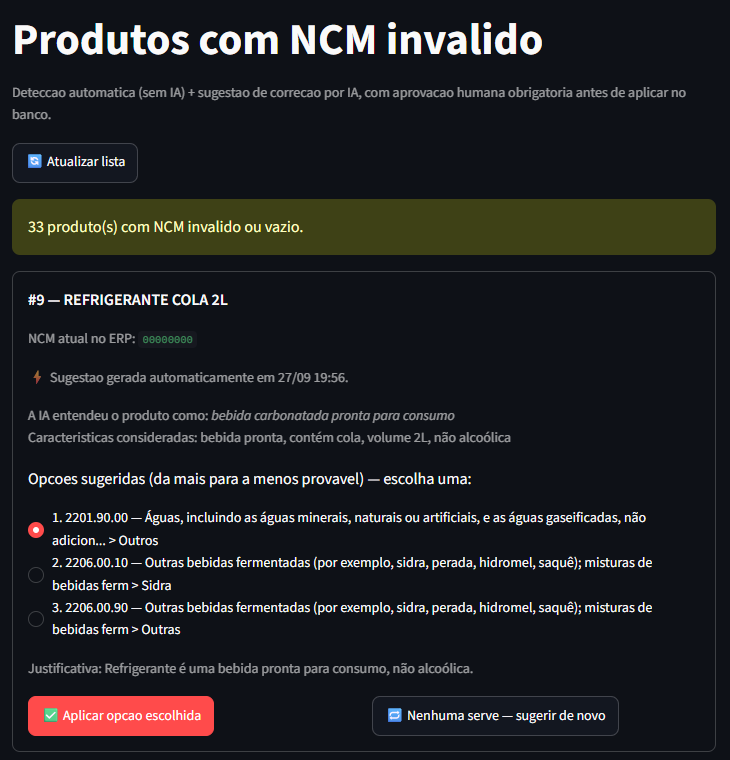
\includegraphics[width=11cm]{images/tela_streamlit.png}
    \fonte{O autor (2026).}
\end{figure}

O exemplo da Figura~\ref{fig:tela_streamlit} é um dos erros do conjunto de teste: para um refrigerante de cola, as três opções sugeridas são de águas e de bebidas fermentadas, e não a posição correta, de bebidas não alcoólicas (2202.10.00). É justamente para esse tipo de caso que a aprovação humana existe: o operador percebe que nenhuma opção corresponde ao produto e, em vez de aplicar a sugestão, pede uma nova ou classifica o produto manualmente.

A camada de acesso ao banco impõe duas restrições. Toda consulta de leitura passa por uma função que só aceita comandos \texttt{SELECT}. A gravação passa por outra função, que só aceita comandos \texttt{UPDATE} com parâmetros, e é chamada apenas pelo botão de aprovação da interface, com um comando fixo: \texttt{UPDATE PRODUTO SET NCM = ? WHERE CODIGO = ?}. Como o código gravado é sempre um dos códigos existentes na tabela, apresentados ao operador, não há como o sistema gravar um código inventado. Por controlar alterações no banco de produção, a interface é servida apenas para o próprio computador (\textit{localhost}).

\section{Evolução das Versões}
\label{sec:evolucao}

A arquitetura final resultou de uma sequência de versões, cada uma motivada pelos erros da anterior. O Quadro~\ref{qua:versoes} resume essa evolução; os resultados quantitativos são apresentados no Capítulo~\ref{cap:resultados}.

\begin{quadro}[H]
\centering
\caption{Versões do processo de sugestão avaliadas}
\label{qua:versoes}
\begin{tabular}{|p{3.3cm}|p{6.2cm}|p{4.7cm}|}
\hline
\textbf{Versão} & \textbf{Funcionamento} & \textbf{Situação} \\
\hline
Agente com ferramentas & LLM decide quais ferramentas chamar (busca na tabela, listagem de subcódigos, consulta ao banco) e em que ordem & Descartada: lenta, instável e com alucinações \\
\hline
Busca com \textit{embeddings} & Busca semântica por vetores somada à busca lexical & Descartada: não aproximou o vocabulário comercial do técnico \\
\hline
Busca e escolha & Busca lexical e duas escolhas restritas do LLM; primeiro com uma opção, depois com três & Base da versão final \\
\hline
Navegação hierárquica & LLM navega capítulo, posição e item vendo a lista completa de cada nível & Descartada: mais lenta e menos precisa \\
\hline
Busca e escolha revisada (1ª fase) & Busca e escolha, com análise do produto, pergunta ao operador, memória e nova tentativa & Base da segunda fase \\
\hline
Dicas de posição e hipóteses & LLM sugere posições prováveis e interpretações alternativas, buscadas também & Descartadas: pioraram ou não alteraram o acerto \\
\hline
Final (2ª fase) & Busca e escolha revisada, com Qwen3 8B, expansão de abreviações, Nota 2 da Seção XVII e base de conhecimento & Adotada \\
\hline
\end{tabular}
\fonte{O autor (2026).}
\end{quadro}

A primeira versão seguiu o projeto: um agente LangChain com o Llama 3.1 8B, que recebia ferramentas para consultar o banco do ERP e a tabela NCM e decidia, em várias rodadas, quais chamar. Na prática, cada classificação exigia de três a cinco chamadas sequenciais ao modelo, o que tornava a resposta lenta e expunha a instabilidade do servidor local sob uso repetido. Mais grave, o modelo nem sempre usava as ferramentas como instruído: em um dos testes, classificou um azulejo de banheiro como ``tubo de escape'', código que não tinha relação com nenhum resultado de busca. Esse comportamento levou à decisão de inverter o controle: o programa executa a busca de forma determinística e o modelo apenas escolhe, com a resposta restrita aos candidatos.

Em paralelo, testou-se a busca semântica com dois modelos de \textit{embeddings} (nomic-embed-text e paraphrase-multilingual-mpnet-base-v2), para encontrar itens sem palavras em comum com a descrição. Os vetores não aproximaram de forma útil o vocabulário comercial do técnico (``azulejo'' de ``ladrilho'', ``bateria'' de ``acumulador''), e o uso de um segundo modelo obrigava o Ollama a alternar modelos na memória de vídeo a cada sugestão, o que travava o servidor. A expansão por sinônimos da WordNet, mais simples, foi adotada no lugar.

A versão de busca e escolha inicialmente devolvia uma única opção. A análise de erros mostrou que, quando o modelo errava, a resposta certa costumava estar entre os primeiros candidatos do mesmo capítulo (leite integral e desnatado, pilha AA e C), o que motivou a apresentação de três opções ao operador.

A navegação hierárquica foi testada para eliminar a dependência da busca: em vez de escolher entre candidatos, o modelo via a lista completa dos 96 capítulos, depois todas as posições do capítulo escolhido e, por fim, todos os itens das posições escolhidas, como faria um classificador humano seguindo as Regras Gerais de Interpretação. Apesar de acertar o capítulo com frequência, essa versão errou mais na escolha final e foi mais lenta, como mostra o Capítulo~\ref{cap:resultados}. A primeira fase terminou com o retorno à busca e escolha, incorporando as melhorias que funcionam independentemente da forma de navegação: a análise do produto com características, a pergunta ao operador, a memória de classificações e a nova tentativa em caso de resposta fora do formato.

A segunda fase partiu dessa versão e foi conduzida sobre os conjuntos de desenvolvimento dev e DEV2. A análise dos erros no DEV2 mostrou três problemas principais: abreviações mal interpretadas, peças de uso geral classificadas como partes de veículos e o código correto ausente dos candidatos. Os dois primeiros motivaram a expansão de abreviações e a inclusão da Nota 2 da Seção XVII. Para o terceiro, foram testadas duas formas de dar ao modelo mais candidatos: pedir a ele as posições de quatro dígitos mais prováveis, cujos itens eram acrescentados à lista, e pedir interpretações alternativas do produto, buscadas também. Ambas pioraram ou não alteraram o acerto e foram descartadas. O modelo Qwen3 8B, disponível nessa fase, substituiu o Qwen2.5 7B por interpretar melhor os produtos (``água sanitária'' passou a ser reconhecida como produto de desinfecção, e ``serrote'', como ferramenta de corte de madeira). Por fim, a base de conhecimento das duas lojas permitiu tratar a falta de candidatos e a escolha fina nos produtos automotivos, que são o foco do ERP.

\chapter{RESULTADOS E DISCUSSÃO}
\label{cap:resultados}

Este capítulo apresenta os resultados em duas partes. A primeira trata da detecção: de códigos inválidos, por consulta à tabela, e de códigos válidos, porém incorretos, com o auxílio do modelo de linguagem. A segunda trata da sugestão: a comparação entre modelos e entre versões no desenvolvimento, a contribuição do modelo de linguagem em relação à busca sem ele, o resultado da versão final no conjunto de teste e a análise dos erros. Ao final, os resultados são confrontados com as metas do projeto e discutidos, incluindo as limitações da avaliação.

\section{Detecção de NCM Inválido}

A Tabela~\ref{tab:invalidos} apresenta o resultado da detecção nos casos rotulados por categoria. Todos os 25 códigos inválidos foram apontados, e nenhum dos 168 códigos válidos foi apontado indevidamente.

\begin{table}[H]
\centering
\caption{Detecção de NCM inválido por categoria}
\label{tab:invalidos}
\begin{tabular}{p{5.2cm} p{5.4cm} c}
\hline
\textbf{Categoria} & \textbf{Exemplos (formato do ERP)} & \textbf{Apontados} \\
\hline
Vazio & vazio, só espaços & 3/3 \\
Só zeros & 00000000, 0 & 4/4 \\
Malformado & 8708100, 870810000, 87O81000 & 8/8 \\
Bem formado e inexistente & 87081099, 99999999 & 8/8 \\
Extinto em atualização da tabela & 39233000, 94032000 & 2/2 \\
\hline
Válido (falso positivo) & códigos dos conjuntos de avaliação & 0/168 \\
\hline
\end{tabular}
\fonte{O autor (2026).}
\end{table}

Nas bases reais das duas lojas, a detecção encontrou 14 mercadorias com código só de zeros e 2 com código de nove dígitos na Loja A, e 54 com código só de zeros e 5 com o campo vazio na Loja B. Nenhuma das 41.606 mercadorias com código válido foi apontada. Esses resultados eram esperados, pois a detecção é uma consulta determinística à tabela oficial; seu valor está em cobrir todas as formas de código inválido, inclusive os extintos, sem custo de modelo de linguagem e sem falsos positivos. Após a restrição aos itens cadastrados como mercadoria, nenhum serviço com código NBS foi apontado como erro; antes dessa restrição, um código NBS válido havia sido indicado incorretamente como NCM inexistente, o que motivou o ajuste.

Os números também mostram o limite dessa verificação: nas bases reais, os códigos inválidos são raros (75 em mais de 41 mil mercadorias), enquanto o erro real mais frequente encontrado, o código ``coringa'' da Loja B, é um código válido e passaria despercebido por ela.

\section{Detecção de NCM Possivelmente Incorreto}

A Tabela~\ref{tab:regras_deteccao} apresenta as regras de decisão avaliadas no DEV2, com os erros plantados, e nos casos reais da Loja B. A regra adotada foi escolhida no DEV2. Dos 98 casos previstos no DEV2, um (o produto ``BOBINA DE IGNICAO'' com NCM errado) não foi medido por falha de execução, o que resulta em 97 casos.

\begin{table}[H]
\centering
\caption{Regras de detecção de NCM incorreto nos conjuntos de desenvolvimento}
\label{tab:regras_deteccao}
\small
\begin{tabular}{p{5.9cm} c c c c}
\hline
 & \multicolumn{2}{c}{\textbf{DEV2 (97 casos)}} & \multicolumn{2}{c}{\textbf{Loja B (80 casos)}} \\
\textbf{Regra} & \textbf{Acurácia} & \textbf{Alarme falso} & \textbf{Acurácia} & \textbf{Alarme falso} \\
\hline
Fora das 3 opções sugeridas & 84,5\% & 30,6\% & 81,2\% & 37,5\% \\
Modelo considera incompatível & 85,6\% & 18,4\% & 85,0\% & 30,0\% \\
Fora das 3 opções e (incompatível ou comparação contra) & 88,7\% & 20,4\% & 85,0\% & 30,0\% \\
\textbf{Fora das 3 opções e incompatível (adotada)} & \textbf{86,6\%} & \textbf{16,3\%} & \textbf{88,8\%} & \textbf{22,5\%} \\
\hline
\end{tabular}
\fonte{O autor (2026). Alarme falso: produtos com NCM correto apontados como suspeitos.}
\end{table}

No DEV2, a regra adotada apontou todos os erros de troca (19/19) e de capítulo (16/16), mas apenas 8 dos 13 erros de vizinho, em que o código errado é outro item da mesma posição, como 8204.12.00 no lugar de 8204.11.00. Esse é o erro mais difícil, pois os dois textos oficiais diferem em um detalhe que a descrição muitas vezes não informa. A regra com a comparação lado a lado detectou mais erros de vizinho (12/13), mas com mais alarmes falsos, e foi preterida. O voto da base de conhecimento não melhorou nenhuma regra: as combinações com ele empataram com as combinações sem ele.

Nos casos reais da Loja B, a regra adotada apontou os 40 produtos cadastrados com o código ``coringa'' de para-choques, como emblemas, correias, retentores e juntas de motor. Entre os 40 produtos presumidos corretos, 9 foram apontados. A inspeção desses alarmes mostrou que ao menos dois parecem ser erros reais da loja, e não do sistema: um coxim de radiador classificado como parte de caixa de câmbio (8708.40.90) e um cilindro auxiliar de embreagem classificado como parte de freio (8708.30.90), quando a NCM possui item próprio para embreagens (8708.93.00). Outros alarmes decorreram de abreviações não expandidas, como ``PRF SXTV'' (parafuso sextavado).

No TESTE2, com 50 produtos com o NCM correto e 50 com erros plantados, a regra adotada foi medida uma única vez e obteve acurácia de 86,0\%, com alarme falso de 6,0\% (3 dos 50 produtos corretos). Foram apontados 39 dos 50 erros (78,0\%): todos os erros de troca (20/20), 14 dos 15 erros de capítulo e apenas 5 dos 15 erros de vizinho, o que confirma a dificuldade observada no desenvolvimento. Entre as regras não adotadas, a que inclui a comparação lado a lado teria apontado mais erros de vizinho (10/15), com acurácia de 88,0\% e alarme falso de 14,0\%; a escolha, feita no desenvolvimento, não foi alterada após a medição. A regra adotada privilegia, portanto, poucos alarmes falsos, o que é desejável em uma verificação que percorre todo o cadastro, em troca de deixar passar parte dos erros mais sutis.

O tempo da verificação ficou entre 17 e 25 segundos por produto, pois inclui a sugestão completa e uma pergunta adicional ao modelo.

\section{Comparação entre Modelos de Linguagem}

A comparação inicial entre modelos foi feita no conjunto dev15, nas primeiras versões da arquitetura de busca e escolha, quando o sistema ainda devolvia uma única opção. A Tabela~\ref{tab:modelos} apresenta o acerto de cada modelo na mesma versão do processo.

\begin{table}[H]
\centering
\caption{Acerto da opção única por modelo no conjunto dev15}
\label{tab:modelos}
\begin{tabular}{p{7.5cm} c c}
\hline
\textbf{Versão do processo} & \textbf{Llama 3.1 8B} & \textbf{Qwen2.5 7B} \\
\hline
Busca e escolha, versão inicial & 9/15 (60,0\%) & 11/15 (73,3\%) \\
Busca e escolha, após ajustes no conjunto dev15 & 10/15 (66,7\%) & 13/15 (86,7\%) \\
\hline
\end{tabular}
\fonte{O autor (2026).}
\end{table}

O Qwen2.5 7B superou o Llama 3.1 8B nas duas versões, com tempo semelhante, e foi adotado na primeira fase. Na inspeção das respostas, ele demonstrou melhor compreensão das descrições em português e seguiu com mais consistência as regras do \textit{prompt}. Esses números, contudo, são otimistas: quando a versão que atingiu 86,7\% no dev15 foi medida pela primeira vez no conjunto teste, acertou a opção única em apenas 14 de 33 produtos (42,4\%), diferença que ilustra o superajuste discutido na seção~\ref{sec:avaliacao}.

Na segunda fase, com o processo final e os mesmos recursos (expansão de abreviações e Nota 2 da Seção XVII), o Qwen3 8B acertou 52,2\% em primeiro lugar e 67,8\% entre as três opções nos 90 produtos de desenvolvimento, contra 47,2\% e 59,6\% do Qwen2.5 7B, com 14,5 segundos por produto. O Qwen3 foi usado sem o modo de raciocínio explícito, para manter o tempo compatível com o uso diário; o efeito desse modo sobre o acerto não foi avaliado.

\section{Evolução das Versões no Desenvolvimento}

A Tabela~\ref{tab:versoes_fase1} resume a primeira fase, com o Qwen2.5 7B. A versão revisada de busca e escolha foi adotada por não piorar em nenhum conjunto e por acrescentar a análise do produto, a pergunta ao operador e a memória; a navegação hierárquica, que acertava mais o capítulo, acumulou erros nos níveis seguintes e foi mais lenta.

\begin{table}[H]
\centering
\caption{Versões da primeira fase com o Qwen2.5 7B}
\label{tab:versoes_fase1}
\begin{tabular}{p{3.6cm} c c c c c c}
\hline
 & \multicolumn{3}{c}{\textbf{dev (41 produtos)}} & \multicolumn{3}{c}{\textbf{teste (33 produtos)}} \\
\textbf{Versão} & \textbf{1º lugar} & \textbf{Top-3} & \textbf{Tempo} & \textbf{1º lugar} & \textbf{Top-3} & \textbf{Tempo} \\
\hline
Busca e escolha & 53,7\% & 61,0\% & 14,5 s & 48,5\% & 63,6\% & $\approx$14 s \\
Navegação hierárquica & 46,3\% & 63,4\% & 22,1 s & 36,4\% & 54,5\% & 65,0 s \\
Busca e escolha revisada & 58,5\% & 70,7\% & 12,9 s & 48,5\% & 63,6\% & 13,2 s \\
\hline
\end{tabular}
\fonte{O autor (2026). Top-3: código correto entre as três opções apresentadas.}
\end{table}

A Tabela~\ref{tab:versoes_fase2} mostra a contribuição de cada recurso da segunda fase nos 90 produtos de desenvolvimento (dev e DEV2). A linha de partida soma os resultados da versão revisada da primeira fase nos dois conjuntos.

\begin{table}[H]
\centering
\caption{Contribuição de cada recurso na segunda fase (dev + DEV2, 90 produtos)}
\label{tab:versoes_fase2}
\begin{tabular}{p{9.2cm} c c}
\hline
\textbf{Configuração} & \textbf{1º lugar} & \textbf{Top-3} \\
\hline
Versão revisada da 1ª fase (Qwen2.5 7B) & 51,1\% & 63,3\% \\
Qwen3 8B + expansão de abreviações & 52,2\% & 64,4\% \\
+ Nota 2 da Seção XVII & 52,2\% & 67,8\% \\
+ base de conhecimento (candidatos e exemplos ao modelo) & 63,3\% & 72,2\% \\
+ NCM mais votado em 1º lugar quando a base é confiante (\textbf{final}) & \textbf{64,4\%} & \textbf{75,6\%} \\
\hline
\end{tabular}
\fonte{O autor (2026).}
\end{table}

O maior ganho veio da base de conhecimento, e ele se concentrou nos produtos automotivos: nos 31 produtos automotivos do desenvolvimento, o acerto passou de 58\% para 90\% em primeiro lugar e de 71\% para 97\% entre as três opções, enquanto nos 59 produtos de outros setores ficou praticamente igual, já que as duas lojas vendem autopeças. As tentativas descartadas na segunda fase são descritas no Capítulo~\ref{cap:desenvolvimento}.

A base de conhecimento também foi avaliada sozinha, sem modelo de linguagem, dentro das próprias lojas, consultando 80\% dos produtos para classificar os outros 20\%. Na Loja A, o NCM mais votado estava correto em 66,5\% dos casos e entre os três mais votados em 80,2\%; na Loja B, em 64,7\% e 83,4\%. Quando uma loja consultava apenas a outra, o acerto caía para 46,3\% e 65,5\% (Loja A consultando a Loja B) e 31,1\% e 47,0\% (Loja B consultando a Loja A). O conhecimento mais valioso, portanto, é o da própria empresa, o que reforça o papel da memória de classificações à medida que o operador aprova sugestões.

\section{Contribuição do Modelo de Linguagem}

Para isolar a contribuição do LLM, as mesmas medições foram feitas sem nenhuma chamada ao modelo: com a busca lexical sozinha (BM25 com sinônimos e fusão RRF da descrição original e da expandida), com a base de conhecimento sozinha e com as duas combinadas, completando as três opções do voto da base com os primeiros resultados da busca. A Tabela~\ref{tab:sem_llm} compara essas linhas de base com a versão final.

\begin{table}[H]
\centering
\caption{Acerto com e sem o modelo de linguagem}
\label{tab:sem_llm}
\begin{tabular}{p{6.0cm} c c c c}
\hline
 & \multicolumn{2}{c}{\textbf{dev + DEV2 (90)}} & \multicolumn{2}{c}{\textbf{TESTE2 (50)}} \\
\textbf{Método} & \textbf{1º lugar} & \textbf{Top-3} & \textbf{1º lugar} & \textbf{Top-3} \\
\hline
Busca lexical, sem LLM & 32,2\% & 54,4\% & 20,0\% & 30,0\% \\
Base de conhecimento, sem LLM & 25,6\% & 34,4\% & 26,0\% & 36,0\% \\
Base de conhecimento + busca, sem LLM & 35,6\% & 51,1\% & 28,0\% & 46,0\% \\
\textbf{Versão final, com LLM} & \textbf{64,4\%} & \textbf{75,6\%} & \textbf{48,0\%} & \textbf{58,0\%} \\
\hline
\end{tabular}
\fonte{O autor (2026).}
\end{table}

No conjunto de teste, a versão final acertou em primeiro lugar 48,0\% dos produtos, contra 20,0\% da busca sozinha e 28,0\% da melhor combinação sem modelo: como a versão final também consulta a base de conhecimento, a comparação justa é com esta última, em relação à qual o LLM acrescentou 20 pontos percentuais em primeiro lugar e 12 pontos entre as três opções. A diferença tem duas origens. A primeira é a escolha: a busca devolve dezenas de candidatos, muitos de palavras coincidentes, e o modelo identifica entre eles o que corresponde ao produto. A segunda é a análise do produto: a descrição técnica gerada pelo modelo leva a busca a itens que a descrição original não alcança; com ela e com a base de conhecimento, o código correto esteve entre os candidatos entregues ao modelo em 78,0\% dos produtos de teste, contra 62,0\% entre os 40 primeiros resultados da busca sozinha. A busca e a base de conhecimento continuam indispensáveis, pois limitam as respostas a códigos existentes e trazem os candidatos, mas o ganho de 20 pontos em primeiro lugar mostra que a escolha feita pelo modelo alcança um acerto que elas, sozinhas, não alcançam.

\section{Resultado da Versão Final no Conjunto de Teste}

A versão final foi medida uma única vez no TESTE2, depois de todas as decisões de desenvolvimento. A Tabela~\ref{tab:teste2} apresenta o resultado, ao lado da medição de referência da versão da primeira fase, feita antes de qualquer alteração. As respostas para cada produto estão no Apêndice~\ref{ap:respostas}.

\begin{table}[H]
\centering
\caption{Resultado no conjunto de teste TESTE2 (50 produtos)}
\label{tab:teste2}
\begin{tabular}{p{6.4cm} c c}
\hline
\textbf{Métrica} & \textbf{Versão da 1ª fase} & \textbf{Versão final} \\
\hline
Acerto em 1º lugar & 32,0\% & 48,0\% \\
Acerto entre as 3 opções & 48,0\% & 58,0\% \\
Código correto entre os candidatos da busca & 64,0\% & 78,0\% \\
Capítulo correto & -- & 72,0\% \\
Tempo médio por produto & 13,4 s & 13,7 s \\
\hline
\end{tabular}
\fonte{O autor (2026).}
\end{table}

O resultado no teste é inferior ao do desenvolvimento (64,4\% e 75,6\%), diferença esperada, pois os recursos da segunda fase foram escolhidos observando os erros dos conjuntos de desenvolvimento. Ainda assim, a versão final melhorou em 16 pontos percentuais o acerto em primeiro lugar e em 10 pontos o acerto entre as três opções em relação à versão da primeira fase, sem aumento de tempo.

O resultado varia fortemente com o setor do produto. Nos 18 produtos automotivos do TESTE2, a versão final acertou 15 em primeiro lugar (83,3\%), e os mesmos 15 entre as três opções; nos 32 produtos de outros setores, acertou 9 em primeiro lugar (28,1\%) e 14 entre as três opções (43,8\%). A base de conhecimento, formada apenas por autopeças, explica boa parte dessa diferença, e o resultado automotivo é o mais representativo do uso real do Lux Auto, voltado a oficinas mecânicas.

\section{Análise dos Erros da Versão Final}

Na versão final, o código correto ficou fora das três opções em 21 dos 50 produtos de teste. A Tabela~\ref{tab:erros} classifica esses erros pelo nível da hierarquia em que ocorreram.

\begin{table}[H]
\centering
\caption{Erros da versão final no TESTE2, por nível da hierarquia}
\label{tab:erros}
\begin{tabular}{p{4.4cm} c p{8.6cm}}
\hline
\textbf{Tipo de erro} & \textbf{Casos} & \textbf{Produtos} \\
\hline
Item errado na posição correta & 6 & bronzina de biela, multímetro, bola de basquete, aspirador de pó, frango congelado, teclado USB \\
Posição errada no capítulo correto & 1 & sal refinado \\
Capítulo errado & 14 & calota, jaqueta de couro, mesa de jantar, fogão, colchão, mochila, \textit{pendrive}, aparelho de barbear, vestido, fita isolante, esmalte, amaciante, lençol, \textit{mouse} \\
\hline
\textbf{Total} & \textbf{21} & \\
\hline
\end{tabular}
\fonte{O autor (2026).}
\end{table}

Diferentemente da primeira fase, em que metade dos erros ocorria no último nível, a maior parte dos erros restantes é de capítulo, e em 11 dos 21 casos o código correto nem chegou aos candidatos da busca. São produtos cujo nome comercial está longe do texto oficial ou cuja classificação depende de uma regra da tabela, e não do nome: a jaqueta de couro foi classificada como vestuário de tecido, pois a NCM a classifica entre as obras de couro (42.03); a mesa de jantar, como utensílio de madeira para mesa, e não como móvel; o \textit{pendrive}, como unidade de memória de computador (84.71), quando a NCM o classifica entre os suportes de armazenamento (85.23); o \textit{mouse}, como aparelho elétrico genérico, e não como periférico de computador; e a fita isolante, como fita de tecido com borracha, e não como fita de plástico (39.19). Nesses casos, a descrição técnica gerada pelo modelo descreveu corretamente o produto, mas não com os termos que levariam a busca à posição certa.

Entre os produtos automotivos, os três erros foram a bronzina de biela, cujo código correto não chegou aos candidatos; a calota, classificada como pneu porque a interpretação do modelo a associou a rodas; e o multímetro, em que o modelo escolheu o item vizinho da mesma posição, que se distingue pela presença de dispositivo registrador. Nos 5 produtos em que o código correto apareceu em segundo lugar, como a banana e o desinfetante, a distinção é entre itens da mesma posição, e a decisão do operador, com o produto em mãos, resolve o caso.

\section{Atendimento às Metas do Projeto}

O projeto estabeleceu como critérios de sucesso uma taxa de detecção de pelo menos 85\% e uma taxa de acerto das correções de pelo menos 75\%; a meta de tempo de até 30 segundos por produto foi adotada depois, como critério de viabilidade. Para os códigos inválidos, objeto da meta de detecção do projeto, ela foi atingida: todos foram detectados, sem falsos positivos. Para os códigos válidos, porém incorretos, que o projeto não previa, o resultado depende do tipo de erro: todos os 40 erros reais da Loja B foram apontados, mas, no conjunto de teste, foram apontados 78,0\% dos erros plantados, abaixo dos 85\%, por causa dos erros entre itens vizinhos de uma mesma posição; a acurácia, considerando também os produtos corretos, foi de 86,0\%, com apenas 6,0\% de alarmes falsos. A meta de tempo também foi atingida nas medições de avaliação, com 13,7 segundos por sugestão e até 25 segundos por verificação.

A meta de acerto das correções foi atingida apenas no recorte automotivo. No conjunto de teste completo, o código correto esteve em primeiro lugar em 48,0\% dos produtos e entre as três opções em 58,0\%, abaixo dos 75\%. Nos produtos automotivos, que correspondem ao uso real do ERP, o acerto foi de 83,3\% em primeiro lugar, acima da meta, mas com apenas 18 produtos, o que torna esse número menos preciso.

Esses números devem ser lidos à luz do fluxo com supervisão humana. Nenhuma sugestão continha código inexistente, já que as respostas são restritas aos códigos da tabela, e nenhum código é gravado sem aprovação. O sistema, portanto, não substitui o conhecimento fiscal do operador ou do suporte, mas reduz o esforço de classificação, impede que o erro mais grave, o código inexistente ou extinto, chegue à emissão da nota e aponta códigos válidos que provavelmente pertencem a outro produto.

\section{Discussão}

Quatro observações gerais emergem dos experimentos. A primeira é que restringir o papel do modelo foi mais eficaz do que ampliar sua autonomia. O agente com ferramentas, mais próximo da proposta original, produziu códigos sem relação com a busca e exigia várias chamadas por produto; a arquitetura de busca e escolha, em que o programa controla o fluxo e o modelo apenas escolhe entre candidatos verificados, eliminou a possibilidade de código inventado e reduziu o tempo e a instabilidade. Esse resultado converge com a recomendação da literatura de usar o LLM como ferramenta de proposição subordinada a mecanismos de verificação e à decisão humana \cite{Natarajan2024AI2L,huang2025hallucination} e com a arquitetura proposta por \citeonline{zhang2026hs} para o SH, em que o fluxo também é fixo e o modelo atua em etapas restritas.

A segunda é que, mesmo restrito, o modelo contribui de forma substancial para o acerto: no teste, a busca combinada com a base de conhecimento, sem modelo, acertou 28\% em primeiro lugar; com ele, 48\%. O papel do modelo não é conhecer a tabela, que ele recebe pronta, mas interpretar a descrição comercial e escolher entre textos técnicos parecidos, justamente a parte que regras e buscas lexicais não resolvem.

A terceira é que exemplos reais valem mais do que ajustes no \textit{prompt}. As alterações de \textit{prompt} e de busca da segunda fase trouxeram ganhos de poucos pontos, enquanto a base de conhecimento elevou o acerto automotivo de 58\% para 90\% no desenvolvimento e resultou em 83\% no teste. Esse resultado aproxima o protótipo dos classificadores supervisionados de NCM \cite{batista2018ncm,pinheiro2022ncm}, que dependem de grandes volumes de exemplos, mas sem treinamento: basta inserir produtos classificados na base. Ao mesmo tempo, o caso da Loja B mostra que exemplos reais trazem erros reais, e que filtrá-los e apontá-los é parte do problema.

A quarta é metodológica: o resultado de 86,7\% no conjunto usado para os primeiros ajustes caiu para 42,4\% em casos novos, e, na segunda fase, o resultado de 75,6\% no desenvolvimento correspondeu a 58,0\% no teste. Sem a separação entre desenvolvimento e teste, o trabalho teria relatado um desempenho substancialmente maior do que o real.

\subsection{Limitações e Ameaças à Validade}

Os resultados devem ser interpretados considerando as seguintes limitações:

\begin{itemize}
    \item \textbf{Tamanho dos conjuntos}: com 50 produtos de teste, cada produto equivale a 2 pontos percentuais, e, no recorte automotivo, a cerca de 6 pontos; diferenças pequenas entre versões não são estatisticamente conclusivas;
    \item \textbf{Gabarito}: a classificação correta foi conferida pelo autor na tabela oficial, e não por um classificador fiscal certificado; em produtos ambíguos, foram aceitos todos os códigos plausíveis;
    \item \textbf{Erros plantados e presumidos}: na detecção de NCM incorreto, os erros do DEV2 e do TESTE2 foram plantados por sorteio, e os produtos considerados corretos da Loja B não foram conferidos um a um, de modo que parte dos alarmes falsos pode corresponder a erros reais;
    \item \textbf{Representatividade das bases}: as duas lojas são do setor de autopeças, o que explica a diferença de desempenho entre setores; a base de conhecimento não representa empresas de outros ramos;
    \item \textbf{Dados fictícios na sugestão}: os produtos dos conjuntos de sugestão foram escritos para os testes, e não extraídos de clientes; descrições reais tendem a ser mais abreviadas e ruidosas;
    \item \textbf{Infraestrutura}: os tempos foram medidos em uma única máquina, e o servidor local de modelos apresentou instabilidades ao longo do trabalho, que podem ter afetado algumas das medições de tempo; além disso, em uma execução do protótipo realizada após a avaliação, com o processo em segundo plano lendo o ERP, cinco de dez verificações levaram mais de 30 segundos (até 42 segundos), o que indica que o tempo em uso real pode superar o medido.
\end{itemize}

\chapter{CONCLUSÃO}
\label{cap:conclusao}

Este trabalho investigou em que medida um modelo de linguagem de pequeno porte, executado localmente e restrito a escolher entre candidatos recuperados da tabela oficial, consegue apontar classificações NCM inválidas ou incorretas no cadastro de produtos de um ERP e sugerir a classificação correta, em tempo compatível com o uso diário e sob supervisão humana. Para responder a essa pergunta, foi desenvolvido e avaliado um protótipo integrado ao ERP Lux Auto, executado inteiramente em um computador convencional, sem custo de API e sem alterações no código ou na estrutura do ERP.

A resposta obtida é positiva para a detecção de códigos inválidos e parcial para a detecção de códigos incorretos e para a sugestão. A detecção de códigos inválidos foi resolvida de forma determinística, sem modelo de linguagem: todos os códigos vazios, malformados, inexistentes e extintos dos casos de avaliação foram apontados, sem nenhum falso positivo entre mais de 41 mil mercadorias reais. A detecção de códigos válidos, porém incorretos, que depende do modelo, teve acurácia de 86,6\% no desenvolvimento e de 88,8\% nos erros reais de uma loja, na qual apontou todos os 40 produtos cadastrados com um código ``coringa''; no conjunto de teste, a acurácia foi de 86,0\%, com 6,0\% de alarmes falsos, mas apenas 78,0\% dos erros plantados foram apontados, pois erros entre itens vizinhos de uma mesma posição continuam difíceis de perceber. Na sugestão, a versão final acertou o código em primeiro lugar em 48,0\% dos produtos de teste e entre as três opções em 58,0\%, em cerca de 14 segundos por produto, abaixo da meta de 75\% no conjunto completo, mas com 83,3\% de acerto em primeiro lugar nos produtos automotivos, foco do ERP. Em todos os casos, nenhuma sugestão continha código inexistente, e nenhum código foi gravado sem aprovação humana.

Os objetivos específicos foram atendidos da seguinte forma: as inconsistências fiscais foram delimitadas a partir da experiência no suporte técnico, e a NCM foi escolhida como foco; a tabela NCM foi estruturada em uma base local com busca textual; o protótipo foi implementado com detecção de códigos inválidos e de códigos possivelmente incorretos, sugestão, execução em segundo plano, notificação e aprovação humana; foram construídos conjuntos separados de desenvolvimento e de teste, incluindo códigos inválidos de diferentes tipos e erros reais de classificação; e o protótipo foi avaliado quanto à detecção, ao acerto e ao tempo, com comparação entre três modelos, entre arquiteturas e contra linhas de base sem modelo de linguagem.

As principais contribuições do trabalho são: uma arquitetura de busca seguida de escolha restrita, na qual o modelo de linguagem não acessa o banco nem pode responder com códigos inexistentes; a medição da contribuição do modelo, que elevou o acerto em primeiro lugar de 28,0\% para 48,0\% em relação à melhor combinação de busca e base de conhecimento sem ele; o uso de produtos já classificados por outras empresas como base de conhecimento, sem treinamento, que elevou substancialmente o acerto no setor automotivo; um método de verificação de códigos válidos que encontrou um erro real e sistemático no cadastro de uma loja; e um protocolo de avaliação com conjunto de teste congelado e medido uma única vez, que mostrou o quanto a avaliação nos próprios casos de ajuste superestima o desempenho.

\section{Trabalhos Futuros}

A partir dos resultados e das limitações observadas, sugerem-se as seguintes continuidades:

\begin{itemize}
    \item \textbf{Demais categorias fiscais}: estender a arquitetura ao CST, ao CFOP e à relação entre Inscrição Estadual e Indicador de Contribuinte, cuja detecção pode, em boa parte, seguir regras determinísticas semelhantes às da NCM;
    \item \textbf{Bases de outros setores}: ampliar a base de conhecimento com empresas de outros ramos, que hoje concentram a maior parte dos erros, e medir o ganho em cada setor;
    \item \textbf{Avaliação com gabarito profissional}: medir o sistema em produtos reais de clientes com o gabarito conferido por um profissional de classificação fiscal, o que permitiria também conferir os alarmes da detecção de NCM incorreto;
    \item \textbf{Vocabulário técnico e notas explicativas}: construir, a partir das aprovações dos operadores, um dicionário de correspondências entre nomes comerciais e termos da NCM, e incorporar à busca as Notas Explicativas do Sistema Harmonizado, atacando os erros de capítulo, que são a maior parte dos erros restantes;
    \item \textbf{Abreviações aprendidas}: ampliar a tabela de abreviações com as encontradas nas bases reais, que causaram parte dos alarmes falsos da detecção;
    \item \textbf{Modelos maiores ou ajustados}: avaliar modelos maiores, quando o hardware permitir, o modo de raciocínio explícito do Qwen3 ou um modelo pequeno ajustado com exemplos de classificação, comparando ganho de acerto e custo de execução;
    \item \textbf{Integração com o ERP}: substituir a consulta periódica por um aviso no próprio ERP no momento do cadastro, caso a desenvolvedora opte por essa integração.
\end{itemize}


% ----------------------------------------------------------
% ELEMENTOS PÓS-TEXTUAIS
% ----------------------------------------------------------
\postextual

% Referências bibliográficas
\bibliography{referencias}

% Apêndices
\begin{apendicesenv}

\chapter{Conjuntos de Casos}
\label{ap:conjuntos}

Este apêndice lista os produtos dos conjuntos utilizados na avaliação da sugestão, com as descrições exatamente como foram fornecidas ao sistema e os códigos NCM aceitos como corretos. Os conjuntos dev15, dev e teste foram usados nas primeiras versões; o DEV2 e o TESTE2 foram sorteados, com semente fixa, de um mesmo grupo de 99 produtos novos, e o TESTE2 foi medido uma única vez, com a versão final.

\begin{center}
\small
\begin{longtable}{r p{7.6cm} p{6.4cm}}
\caption{Conjunto dev15}\label{tab:ap_dev15} \\
\hline
\textbf{Nº} & \textbf{Descrição} & \textbf{NCM aceito(s)} \\
\hline
\endfirsthead
\hline
\textbf{Nº} & \textbf{Descrição} & \textbf{NCM aceito(s)} \\
\hline
\endhead
\hline
\endfoot
1 & vela de ignição & 8511.10.00 \\
2 & amortecedor & 8708.80.00 \\
3 & retrovisor & 7009.10.00 \\
4 & radiador para automóvel & 8708.91.00 \\
5 & para-choque & 8708.10.00 \\
6 & PARACHOQUE & 8708.10.00 \\
7 & farol & 8512.20.11 \\
8 & embreagem & 8708.93.00 \\
9 & pneu novo para carro de passeio & 4011.10.00 \\
10 & correia dentada & 4010.35.00, 4010.36.00 \\
11 & pastilha de freio & 8708.30.19, 8708.30.11, 8708.30.90 \\
12 & disco de freio & 8708.30.19, 8708.30.11, 8708.30.90 \\
13 & óleo lubrificante para motor & 2710.19.31, 2710.19.32 \\
14 & bateria de chumbo para automóvel & 8507.10.10, 8507.10.90 \\
15 & AZULEIJO DE BANHEIRO AZUL & 6907.23.00, 6907.21.00, 6907.22.00 \\
\end{longtable}
\end{center}

\begin{center}
\small
\begin{longtable}{r p{6.6cm} p{4.4cm} p{2.6cm}}
\caption{Conjunto dev}\label{tab:ap_dev} \\
\hline
\textbf{Nº} & \textbf{Descrição cadastrada} & \textbf{NCM aceito(s)} & \textbf{Setor} \\
\hline
\endfirsthead
\hline
\textbf{Nº} & \textbf{Descrição cadastrada} & \textbf{NCM aceito(s)} & \textbf{Setor} \\
\hline
\endhead
\hline
\endfoot
1 & BOMBA D AGUA MOTOR & 8413.30.90 & automotivo \\
2 & ALTERNADOR 12V & 8511.50.10 & automotivo \\
3 & MOTOR DE ARRANQUE & 8511.40.00 & automotivo \\
4 & PARABRISA DIANTEIRO & 7007.21.00, 8708.22.00 & automotivo \\
5 & JUNTA DO CABECOTE & 8484.10.00 & automotivo \\
6 & FILTRO DE OLEO & 8421.23.00 & automotivo \\
7 & CABO DE VELA & 8544.30.00 & automotivo \\
8 & EXTINTOR DE INCENDIO PO QUIMICO & 8424.10.00 & automotivo \\
9 & BUZINA 12V & 8512.30.00 & automotivo \\
10 & PNEU ARO 17 MOTO & 4011.40.00 & automotivo \\
11 & CAMARA DE AR BICICLETA & 4013.20.00 & automotivo \\
12 & FLUIDO DE FREIO DOT 4 & 3819.00.00 & automotivo \\
13 & ADITIVO PARA RADIADOR & 3820.00.00 & automotivo \\
14 & ACUCAR REFINADO 1KG & 1701.99.00 & alimentos \\
15 & OLEO DE SOJA 900ML & 1507.90.11 & alimentos \\
16 & MACARRAO ESPAGUETE 500G & 1902.19.00, 1902.11.00 & alimentos \\
17 & BISCOITO RECHEADO CHOCOLATE & 1905.31.00 & alimentos \\
18 & SUCO DE UVA INTEGRAL 1L & 2009.61.00, 2009.69.00 & bebidas \\
19 & AGUA MINERAL SEM GAS 500ML & 2201.10.00 & bebidas \\
20 & VINHO TINTO SECO 750ML & 2204.21.00 & bebidas \\
21 & PERFUME 100ML & 3303.00.10 & higiene \\
22 & PAPEL TOALHA 2 ROLOS & 4818.20.00 & higiene \\
23 & ESCOVA DE DENTES & 9603.21.00 & higiene \\
24 & FRALDA DESCARTAVEL INFANTIL & 9619.00.00 & higiene \\
25 & MEIA DE ALGODAO & 6115.95.00 & vestuario \\
26 & CUECA BOXER ALGODAO & 6107.11.00 & vestuario \\
27 & CHINELO DE BORRACHA & 6402.20.00 & calcados \\
28 & FONE DE OUVIDO BLUETOOTH & 8518.30.00 & eletronicos \\
29 & MICROONDAS 30L & 8516.50.00 & eletrodomesticos \\
30 & LIQUIDIFICADOR 600W & 8509.40.10 & eletrodomesticos \\
31 & VENTILADOR DE MESA & 8414.51.10 & eletrodomesticos \\
32 & CHAVE DE FENDA & 8205.40.00 & ferramentas \\
33 & ALICATE UNIVERSAL & 8203.20.10 & ferramentas \\
34 & TRENA 5M & 9017.80.10 & ferramentas \\
35 & TIJOLO CERAMICO 8 FUROS & 6904.10.00 & construcao \\
36 & CANO PVC 100MM & 3917.23.00 & construcao \\
37 & FIO ELETRICO 2,5MM & 8544.49.00 & construcao \\
38 & LAPIS PRETO & 9609.10.00 & papelaria \\
39 & SOFA 3 LUGARES & 9401.61.00, 9401.71.00 & moveis \\
40 & BICICLETA ARO 29 & 8712.00.10 & esporte \\
41 & RACAO PARA CAES 15KG & 2309.10.00 & pet \\
\end{longtable}
\end{center}

\begin{center}
\small
\begin{longtable}{r p{6.6cm} p{4.4cm} p{2.6cm}}
\caption{Conjunto teste}\label{tab:ap_teste} \\
\hline
\textbf{Nº} & \textbf{Descrição cadastrada} & \textbf{NCM aceito(s)} & \textbf{Setor} \\
\hline
\endfirsthead
\hline
\textbf{Nº} & \textbf{Descrição cadastrada} & \textbf{NCM aceito(s)} & \textbf{Setor} \\
\hline
\endhead
\hline
\endfoot
1 & ARROZ BRANCO TIPO 1 5KG & 1006.30.21 & alimentos \\
2 & CAFE TORRADO E MOIDO 500G & 0901.21.00 & alimentos \\
3 & REFRIGERANTE COLA 2L & 2202.10.00 & bebidas \\
4 & CERVEJA LATA 350ML & 2203.00.00 & bebidas \\
5 & LEITE UHT INTEGRAL 1L & 0401.20.10 & alimentos \\
6 & CHOCOLATE AO LEITE BARRA 90G & 1806.32.10 & alimentos \\
7 & DETERGENTE LIQUIDO LAVA LOUCAS 500ML & 3402.50.00 & limpeza \\
8 & SABONETE EM BARRA 90G & 3401.11.90 & higiene \\
9 & SHAMPOO ANTICASPA 350ML & 3305.10.00 & higiene \\
10 & CREME DENTAL 90G & 3306.10.00 & higiene \\
11 & PAPEL HIGIENICO FOLHA DUPLA 12 ROLOS & 4818.10.00 & higiene \\
12 & CAMISETA ALGODAO MASCULINA & 6109.10.00 & vestuario \\
13 & CALCA JEANS FEMININA & 6204.62.00 & vestuario \\
14 & TENIS ESPORTIVO & 6404.11.00, 6402.19.00 & calcados \\
15 & TOALHA DE BANHO ALGODAO & 6302.60.00 & cama mesa banho \\
16 & CELULAR SMARTPHONE 128GB & 8517.13.00 & eletronicos \\
17 & NOTEBOOK 15 POLEGADAS & 8471.30.12, 8471.30.19 & eletronicos \\
18 & GELADERA FROST FREE DUPLEX & 8418.10.00 & eletrodomesticos \\
19 & LAMPADA LED 9W & 8539.52.00 & eletricos \\
20 & PILHA ALCALINA AA & 8506.10.19 & eletricos \\
21 & MARTELO DE UNHA CABO MADEIRA & 8205.20.00 & ferramentas \\
22 & FURADERA ELETRICA 500W & 8467.21.00 & ferramentas \\
23 & CIMENTO PORTLAND 50KG & 2523.29.10 & construcao \\
24 & TINTA ACRILICA PAREDE 18L & 3209.10.10 & construcao \\
25 & PARAFUSO SEXTAVADO ACO M8 & 7318.15.00 & ferragens \\
26 & CADERNO ESPIRAL 96 FOLHAS & 4820.20.00 & papelaria \\
27 & CANETA ESFEROGRAFICA AZUL & 9608.10.00 & papelaria \\
28 & CADEIRA DE ESCRITORIO GIRATORIA & 9401.31.00, 9401.39.00 & moveis \\
29 & BOLA DE FUTEBOL & 9506.62.00 & esporte \\
30 & FILTRO DE AR DO MOTOR & 8421.31.00 & automotivo \\
31 & OLEO MOTOR 5W30 1L & 2710.19.32 & automotivo \\
32 & LAMPADA FAROL H4 12V & 8539.21.10 & automotivo \\
33 & BATERIA 60AH 12V & 8507.10.90 & automotivo \\
\end{longtable}
\end{center}

\begin{center}
\small
\begin{longtable}{r p{6.6cm} p{4.4cm} p{2.6cm}}
\caption{Conjunto DEV2}\label{tab:ap_dev2} \\
\hline
\textbf{Nº} & \textbf{Descrição cadastrada} & \textbf{NCM aceito(s)} & \textbf{Setor} \\
\hline
\endfirsthead
\hline
\textbf{Nº} & \textbf{Descrição cadastrada} & \textbf{NCM aceito(s)} & \textbf{Setor} \\
\hline
\endhead
\hline
\endfoot
1 & PORCA SEXTAVADA M10 & 7318.16.00 & automotivo \\
2 & FUSIVEL LAMINA 10A & 8536.10.00 & automotivo \\
3 & MANG SUP RADIADOR & 4009.31.00, 4009.32.10, 4009.32.90, 8708.91.00 & automotivo \\
4 & SILENCIOSO TRASEIRO ESCAPAMENTO & 8708.92.00 & automotivo \\
5 & BOBINA DE IGNICAO & 8511.30.20 & automotivo \\
6 & MACACO HIDRAULICO GARRAFA 2T & 8425.42.00 & automotivo \\
7 & RELE AUXILIAR 12V 4 TERMINAIS & 8536.41.00 & automotivo \\
8 & JOGO DE ANEIS DE SEGMENTO & 8409.91.16 & automotivo \\
9 & ROLAM RODA DIANT & 8482.10.10, 8482.10.90 & automotivo \\
10 & PALHETA LIMPADOR PARABRISA 20 POL & 8512.90.00 & automotivo \\
11 & PISTAO MOTOR STD & 8409.91.20 & automotivo \\
12 & ALICATE DE PRESSAO & 8203.20.90 & automotivo \\
13 & CIL MESTRE FREIO & 8708.30.90 & automotivo \\
14 & CORREIA DO ALTERNADOR & 4010.31.00, 4010.32.00, 4010.33.00, 4010.34.00 & automotivo \\
15 & PIVO SUSP INF & 8708.80.00 & automotivo \\
16 & BIELETA BARRA ESTABILIZADORA & 8708.80.00 & automotivo \\
17 & TERMINAL DE DIRECAO LD & 8708.94.90, 8708.80.00 & automotivo \\
18 & PASTILHA DE FREIO DIANTEIRA CERAMICA & 8708.30.19 & automotivo \\
19 & ABSORVENTE HIGIENICO & 9619.00.00 & higiene \\
20 & OVOS BRANCOS DUZIA & 0407.21.00 & alimentos \\
21 & KETCHUP 400G & 2103.20.10 & alimentos \\
22 & BATEDEIRA & 8509.40.20 & eletrodomesticos \\
23 & FARINHA DE TRIGO 1KG & 1101.00.10 & alimentos \\
24 & AGUA SANITARIA 1L & 2828.90.11 & limpeza \\
25 & LIXA DAGUA 220 & 6805.20.00 & construcao \\
26 & SERROTE & 8202.10.00 & ferramentas \\
27 & PATINHO BOVINO KG & 0201.30.00, 0202.30.00 & alimentos \\
28 & ACHOCOLATADO EM PO 400G & 1806.10.00, 1806.90.00 & alimentos \\
29 & CAFE SOLUVEL 100G & 2101.11.10 & alimentos \\
30 & SARDINHA EM LATA 125G & 1604.13.10 & alimentos \\
31 & SABAO EM PO 1KG & 3402.50.00 & limpeza \\
32 & SERRA CIRCULAR & 8467.22.00 & ferramentas \\
33 & PROTETOR SOLAR FPS 50 & 3304.99.90 & higiene \\
34 & VARA DE PESCA & 9507.10.00 & esporte \\
35 & BOTA DE SEGURANCA BICO DE ACO & 6403.40.00 & calcados \\
36 & MAIONESE 500G & 2103.90.11 & alimentos \\
37 & MANTEIGA COM SAL 200G & 0405.10.00 & alimentos \\
38 & BORRACHA ESCOLAR & 4016.92.00 & papelaria \\
39 & CHAVE INGLESA & 8204.12.00 & ferramentas \\
40 & IOGURTE NATURAL 170G & 0403.20.00 & alimentos \\
41 & AR CONDICIONADO SPLIT 12000 BTUS & 8415.10.11 & eletrodomesticos \\
42 & TRAVESSEIRO & 9404.90.00 & cama mesa banho \\
43 & FEIJAO CARIOCA 1KG & 0713.33.99 & alimentos \\
44 & ARMARIO DE ACO 2 PORTAS & 9403.20.90, 9403.10.00 & moveis \\
45 & TORNEIRA DE PIA & 8481.80.19 & construcao \\
46 & CAIXA DE SOM BLUETOOTH & 8518.22.00, 8518.21.00 & eletronicos \\
47 & VODKA 1L & 2208.60.00 & bebidas \\
48 & CHUVEIRO ELETRICO & 8516.10.00 & eletrodomesticos \\
49 & DISJUNTOR 20A & 8536.20.00 & construcao \\
\end{longtable}
\end{center}

\begin{center}
\small
\begin{longtable}{r p{6.6cm} p{4.4cm} p{2.6cm}}
\caption{Conjunto TESTE2}\label{tab:ap_teste2} \\
\hline
\textbf{Nº} & \textbf{Descrição cadastrada} & \textbf{NCM aceito(s)} & \textbf{Setor} \\
\hline
\endfirsthead
\hline
\textbf{Nº} & \textbf{Descrição cadastrada} & \textbf{NCM aceito(s)} & \textbf{Setor} \\
\hline
\endhead
\hline
\endfoot
1 & PNEU 175/70 R14 & 4011.10.00 & automotivo \\
2 & FILTRO AR COND CABINE & 8421.39.90 & automotivo \\
3 & BRONZINA DE BIELA & 8483.30.90, 8409.91.90 & automotivo \\
4 & CALOTA ARO 14 & 8708.70.90 & automotivo \\
5 & LAMPADA PINGO 12V 5W & 8539.29.10 & automotivo \\
6 & TAPETE AUTOMOTIVO BORRACHA JOGO & 4016.91.00 & automotivo \\
7 & FILTRO DE COMBUSTIVEL & 8421.23.00 & automotivo \\
8 & CHAVE DE RODA CRUZ & 8204.11.00 & automotivo \\
9 & TAMPA DO RADIADOR & 8708.91.00 & automotivo \\
10 & RETENTOR VIRABREQUIM & 4016.93.00 & automotivo \\
11 & PARAFUSO DE RODA & 7318.15.00 & automotivo \\
12 & MULTIMETRO DIGITAL & 9030.31.00 & automotivo \\
13 & CERA AUTOMOTIVA PASTA & 3405.30.00 & automotivo \\
14 & BOMBA COMBUSTIVEL ELETRICA FLEX & 8413.30.10 & automotivo \\
15 & SOQUETE ENCAIXE 1/2 10MM & 8204.20.00 & automotivo \\
16 & CHAVE COMBINADA 13MM & 8204.11.00 & automotivo \\
17 & ARRUELA LISA ACO 10MM & 7318.22.00 & automotivo \\
18 & SONDA LAMBDA & 9027.10.00 & automotivo \\
19 & JAQUETA DE COURO & 4203.10.00 & vestuario \\
20 & ENERGETICO LATA 250ML & 2202.10.00, 2202.99.00 & bebidas \\
21 & PREGO 17X27 1KG & 7317.00.90 & construcao \\
22 & CARREGADOR DE CELULAR USB & 8504.40.10, 8504.40.90 & eletronicos \\
23 & MESA DE JANTAR MADEIRA & 9403.60.00 & moveis \\
24 & FOGAO 4 BOCAS & 7321.11.00 & eletrodomesticos \\
25 & BANANA PRATA KG & 0803.90.00 & alimentos \\
26 & COLCHAO DE ESPUMA SOLTEIRO & 9404.21.00 & moveis \\
27 & MOCHILA ESCOLAR & 4202.92.00 & papelaria \\
28 & PENDRIVE 32GB & 8523.51.10, 8523.51.90 & eletronicos \\
29 & APARELHO DE BARBEAR DESCARTAVEL & 8212.10.20 & higiene \\
30 & BOLA DE BASQUETE & 9506.62.00 & esporte \\
31 & VESTIDO MALHA ALGODAO & 6104.42.00 & vestuario \\
32 & FITA ISOLANTE & 3919.10.20 & construcao \\
33 & BONECA DE PLASTICO & 9503.00.22 & brinquedos \\
34 & ESMALTE DE UNHA & 3304.30.00 & higiene \\
35 & ARGAMASSA 20KG & 3824.50.00 & construcao \\
36 & SAL REFINADO 1KG & 2501.00.20 & alimentos \\
37 & AMACIANTE ROUPA 2L & 3809.91.90 & limpeza \\
38 & IMPRESSORA MULTIFUNCIONAL JATO DE TINTA & 8443.31.11, 8443.31.19 & eletronicos \\
39 & TELHA FIBROCIMENTO & 6811.82.00 & construcao \\
40 & ASPIRADOR DE PO & 8508.11.00 & eletrodomesticos \\
41 & FERRO DE PASSAR & 8516.40.00 & eletrodomesticos \\
42 & FRANGO INTEIRO CONGELADO & 0207.12.10, 0207.12.20 & alimentos \\
43 & LENCOL CASAL ALGODAO & 6302.21.00, 6302.31.00 & cama mesa banho \\
44 & TOMADA 2P+T & 8536.69.90 & construcao \\
45 & DESINFETANTE 2L & 3808.94.19 & limpeza \\
46 & MOUSE SEM FIO & 8471.60.53 & eletronicos \\
47 & TECLADO USB & 8471.60.52 & eletronicos \\
48 & QUEIJO MUSSARELA FATIADO & 0406.10.10 & alimentos \\
49 & DESODORANTE AEROSOL MASC 150ML & 3307.20.10, 3307.20.90 & higiene \\
50 & MAQUINA DE LAVAR ROUPAS & 8450.11.00 & eletrodomesticos \\
\end{longtable}
\end{center}

\chapter{\textit{Prompts} da Versão Final}
\label{ap:prompts}

Os \textit{prompts} são reproduzidos sem acentuação, como no código-fonte do protótipo. Os exemplos citados neles não pertencem a nenhum conjunto de avaliação.

\section*{\textit{Prompt} da análise do produto}
{\small
\begin{verbatim}
Voce conhece a Nomenclatura Comum do Mercosul (NCM). Para a
descricao de produto recebida (pode ter erro de digitacao),
responda:

- descricao_tecnica: o nome tecnico/formal que a NCM usa para esse
tipo de mercadoria. No maximo 8 palavras. Sem embalagem, volume,
peso, medidas, potencia, cor ou marca.
- caracteristicas: ate 15 palavras com o que decide a
classificacao: material, funcao, aplicacao (ex.: para automovel),
estado (novo, refinado, cru...), se e produto completo ou peca. Se
algo importante nao da para saber pela descricao, diga "nao
informado: ...".

Responda SEMPRE em portugues do Brasil, nunca em outro idioma.

Exemplos:
'TV LED 50 POLEGADAS' -> descricao_tecnica 'aparelho receptor de
televisao'; caracteristicas 'aparelho eletronico completo, tela de
LED, uso domestico'
'GUARDA ROUPA MDF' -> descricao_tecnica 'movel de madeira para
quarto de dormir'; caracteristicas 'movel completo, madeira
aglomerada (MDF), uso domestico'
'SUCO DE LARANJA 1L' -> descricao_tecnica 'suco de laranja nao
fermentado'; caracteristicas 'bebida nao alcoolica, fruta, pronto
para beber; nao informado: valor Brix'
\end{verbatim}
}

\section*{\textit{Prompt} de sistema das escolhas de capítulo e itens}
{\small
\begin{verbatim}
Voce e um especialista em classificacao fiscal de mercadorias na
NCM (Nomenclatura Comum do Mercosul) da Receita Federal.

A descricao do produto vem do jeito que foi digitada no cadastro
de um ERP: pode estar em maiusculas, sem hifen, abreviada ou com
erro de digitacao (ex.: PARACHOQUE = para-choque de carro;
AZULEIJO = azulejo). Os candidatos vem de uma busca automatica e
CONTEM RUIDO: alguns nao tem nada a ver com o produto.

Regras:
1. Pense no que o produto E de fato (material, funcao) antes de
escolher. Uma cor ou palavra solta no nome nao muda o que o
produto e (um azulejo azul continua sendo ceramica, nunca peixe).
2. Se um candidato nomeia diretamente o produto (ex.:
'Para-choques e suas partes' para um parachoque), escolha ele.
3. Nao escolha um item 'Outros'/'Outras' so porque ficou em
duvida: todo 'Outros' pertence a uma posicao especifica (ex.:
'Outros' de tijolos refratarios). Escolha primeiro a posicao que
descreve o produto e so depois o item dentro dela.
4. Responda SOMENTE com codigos/capitulos da lista. Na escolha do
capitulo, use NENHUM apenas se nenhum candidato for sequer do
mesmo tipo de produto.
5. Contexto do negocio: o ERP e de uma oficina mecanica de
automoveis. Quando a descricao nao diz o tipo de veiculo e o mesmo
produto existir para automovel e para moto/bicicleta/trator/trem,
prefira o de automovel. Isso vale so para desempatar -- um produto
que claramente nao e peca de carro (ex.: azulejo) continua sendo
classificado pelo que ele e.
6. Cada justificativa deve ser curta e em linguagem simples. Se a
escolha exata depender de uma informacao que a descricao nao tem
(ex.: tipo de ceramica, absorcao de agua), diga qual informacao
falta -- e justamente por isso as outras opcoes existem.

7. Pecas de uso geral NAO sao classificadas como "partes e
acessorios" de veiculos (87.08), mesmo quando sao de carro (Nota 2
da Secao XVII). Elas tem posicao propria: rolamentos (84.82);
parafusos, porcas e arruelas (73.18); molas (73.20); juntas,
retentores e outros artigos de borracha (40.16); mangueiras de
borracha (40.09); correias (40.10); pneus (40.11); filtros
(84.21); bombas (84.13); pecas de motor (84.09); lampadas (85.39);
reles, fusiveis e interruptores (85.36); velas, bobinas,
alternadores e motores de arranque (85.11); farois, buzinas e
limpadores de para-brisa, com suas partes (85.12); vidros (70.07);
espelhos (70.09); fios e cabos eletricos (85.44); ferramentas
(Cap. 82). Use a 87.08 so para partes proprias de veiculo que nao
tenham posicao especifica (para-choques, freios, suspensao,
radiadores, silenciosos, direcao, rodas).
\end{verbatim}
}

\section*{\textit{Prompt} de sistema da verificação do NCM cadastrado}
{\small
\begin{verbatim}
Voce e um especialista em classificacao fiscal de mercadorias na
NCM (Nomenclatura Comum do Mercosul). Voce revisa cadastros de
produtos de um ERP de oficina mecanica para encontrar NCM errado.

A descricao do produto vem como foi digitada no cadastro: pode
estar abreviada ou com erro de digitacao. Julgue pelo que o
produto E (material, funcao, aplicacao), nao por palavras soltas.

Responda SEMPRE em portugues do Brasil, nunca em outro idioma.
\end{verbatim}
}

\chapter{Respostas da Versão Final no Conjunto de Teste}
\label{ap:respostas}

Este apêndice apresenta, para cada produto do TESTE2, as três opções sugeridas pela versão final e a posição em que o código correto apareceu. A execução completa, com a interpretação do modelo, os capítulos escolhidos e o tempo de cada produto, está disponível no repositório do protótipo, no diretório \texttt{data/avaliacoes}.

\begin{center}
\small
\begin{longtable}{r p{5.2cm} p{3.0cm} p{2.6cm} c}
\caption{Respostas da versão final no conjunto TESTE2}\label{tab:ap_teste2_respostas} \\
\hline
\textbf{Nº} & \textbf{Descrição cadastrada} & \textbf{NCM aceito(s)} & \textbf{Opções sugeridas (em ordem)} & \textbf{Acerto} \\
\hline
\endfirsthead
\hline
\textbf{Nº} & \textbf{Descrição cadastrada} & \textbf{NCM aceito(s)} & \textbf{Opções sugeridas (em ordem)} & \textbf{Acerto} \\
\hline
\endhead
\hline
\endfoot
1 & PNEU 175/70 R14 & 4011.10.00 & 4011.10.00 \newline 4011.20.90 \newline 4011.20.10 & 1º \\
2 & FILTRO AR COND CABINE & 8421.39.90 & 8421.39.90 \newline 8415.20.90 \newline 8415.82.10 & 1º \\
3 & BRONZINA DE BIELA & 8483.30.90, 8409.91.90 & 8483.30.29 \newline 8409.91.11 \newline 8483.10.11 & não \\
4 & CALOTA ARO 14 & 8708.70.90 & 4011.10.00 \newline 4011.90.10 \newline 4011.80.20 & não \\
5 & LAMPADA PINGO 12V 5W & 8539.29.10 & 8539.29.10 \newline 8539.52.00 \newline 8539.32.30 & 1º \\
6 & TAPETE AUTOMOTIVO BORRACHA JOGO & 4016.91.00 & 4016.91.00 \newline 4016.10.10 \newline 4011.10.00 & 1º \\
7 & FILTRO DE COMBUSTIVEL & 8421.23.00 & 8421.23.00 \newline 8421.99.99 \newline 8421.29.30 & 1º \\
8 & CHAVE DE RODA CRUZ & 8204.11.00 & 8204.11.00 \newline 8204.12.00 \newline 8205.40.00 & 1º \\
9 & TAMPA DO RADIADOR & 8708.91.00 & 8708.91.00 \newline 8708.99.90 \newline 8708.29.12 & 1º \\
10 & RETENTOR VIRABREQUIM & 4016.93.00 & 4016.93.00 & 1º \\
11 & PARAFUSO DE RODA & 7318.15.00 & 7318.15.00 \newline 7318.14.00 \newline 7318.19.00 & 1º \\
12 & MULTIMETRO DIGITAL & 9030.31.00 & 9030.32.00 \newline 9031.80.40 \newline 9031.90.90 & não \\
13 & CERA AUTOMOTIVA PASTA & 3405.30.00 & 3405.30.00 \newline 3407.00.90 \newline 3404.90.19 & 1º \\
14 & BOMBA COMBUSTIVEL ELETRICA FLEX & 8413.30.10 & 8413.30.10 \newline 8413.91.90 \newline 8413.81.00 & 1º \\
15 & SOQUETE ENCAIXE 1/2 10MM & 8204.20.00 & 8204.20.00 \newline 8204.11.00 \newline 8207.90.00 & 1º \\
16 & CHAVE COMBINADA 13MM & 8204.11.00 & 8204.11.00 \newline 8205.59.00 \newline 8204.12.00 & 1º \\
17 & ARRUELA LISA ACO 10MM & 7318.22.00 & 7318.22.00 \newline 7318.21.00 \newline 7325.99.10 & 1º \\
18 & SONDA LAMBDA & 9027.10.00 & 9027.10.00 \newline 9018.39.29 \newline 9014.80.10 & 1º \\
19 & JAQUETA DE COURO & 4203.10.00 & 6210.30.00 & não \\
20 & ENERGETICO LATA 250ML & 2202.10.00, 2202.99.00 & 2202.10.00 \newline 2206.00.90 \newline 2206.00.10 & 1º \\
21 & PREGO 17X27 1KG & 7317.00.90 & 7317.00.90 \newline 7317.00.10 \newline 7323.10.00 & 1º \\
22 & CARREGADOR DE CELULAR USB & 8504.40.10, 8504.40.90 & 8504.40.10 \newline 8517.62.62 \newline 8517.14.32 & 1º \\
23 & MESA DE JANTAR MADEIRA & 9403.60.00 & 4419.90.00 \newline 4419.20.00 \newline 4419.19.00 & não \\
24 & FOGAO 4 BOCAS & 7321.11.00 & 8516.60.00 & não \\
25 & BANANA PRATA KG & 0803.90.00 & 0803.10.00 \newline 0803.90.00 & 2º \\
26 & COLCHAO DE ESPUMA SOLTEIRO & 9404.21.00 & 3402.90.90 \newline 3402.90.39 \newline 3405.10.00 & não \\
27 & MOCHILA ESCOLAR & 4202.92.00 & 9605.00.00 \newline 9609.20.00 \newline 9616.20.00 & não \\
28 & PENDRIVE 32GB & 8523.51.10, 8523.51.90 & 8471.70.40 & não \\
29 & APARELHO DE BARBEAR DESCARTAVEL & 8212.10.20 & 8510.10.00 \newline 8510.90.11 \newline 8510.90.19 & não \\
30 & BOLA DE BASQUETE & 9506.62.00 & 9506.61.00 \newline 9506.32.00 \newline 9504.90.10 & não \\
31 & VESTIDO MALHA ALGODAO & 6104.42.00 & 6004.90.10 \newline 6006.22.00 \newline 6006.24.00 & não \\
32 & FITA ISOLANTE & 3919.10.20 & 5906.10.00 & não \\
33 & BONECA DE PLASTICO & 9503.00.22 & 9503.00.29 \newline 9503.00.22 \newline 9503.00.21 & 2º \\
34 & ESMALTE DE UNHA & 3304.30.00 & 3208.90.10 \newline 3207.30.00 & não \\
35 & ARGAMASSA 20KG & 3824.50.00 & 3824.50.00 \newline 3824.99.52 \newline 3816.00.90 & 1º \\
36 & SAL REFINADO 1KG & 2501.00.20 & 2530.10.10 \newline 2530.90.90 \newline 2530.90.30 & não \\
37 & AMACIANTE ROUPA 2L & 3809.91.90 & 3405.20.00 & não \\
38 & IMPRESSORA MULTIFUNCIONAL JATO DE TINTA & 8443.31.11, 8443.31.19 & 8443.39.10 \newline 8443.31.11 \newline 8443.32.31 & 2º \\
39 & TELHA FIBROCIMENTO & 6811.82.00 & 6811.82.00 \newline 6810.19.00 \newline 6811.89.00 & 1º \\
40 & ASPIRADOR DE PO & 8508.11.00 & 8508.19.00 \newline 8509.80.90 \newline 8509.40.90 & não \\
41 & FERRO DE PASSAR & 8516.40.00 & 8516.40.00 & 1º \\
42 & FRANGO INTEIRO CONGELADO & 0207.12.10, 0207.12.20 & 0207.27.00 \newline 0210.99.11 & não \\
43 & LENCOL CASAL ALGODAO & 6302.21.00, 6302.31.00 & 5906.10.00 \newline 5911.10.00 & não \\
44 & TOMADA 2P+T & 8536.69.90 & 8536.69.10 \newline 8536.69.90 \newline 8536.90.20 & 2º \\
45 & DESINFETANTE 2L & 3808.94.19 & 3808.94.29 \newline 3808.94.19 \newline 3808.94.22 & 2º \\
46 & MOUSE SEM FIO & 8471.60.53 & 8543.70.35 \newline 8544.49.00 \newline 8543.70.36 & não \\
47 & TECLADO USB & 8471.60.52 & 8471.60.59 \newline 8471.60.53 \newline 8471.60.61 & não \\
48 & QUEIJO MUSSARELA FATIADO & 0406.10.10 & 0406.10.10 \newline 0406.10.90 \newline 0406.90.30 & 1º \\
49 & DESODORANTE AEROSOL MASC 150ML & 3307.20.10, 3307.20.90 & 3307.20.10 \newline 3307.20.90 \newline 3307.49.00 & 1º \\
50 & MAQUINA DE LAVAR ROUPAS & 8450.11.00 & 8450.11.00 \newline 8450.12.00 \newline 8450.20.90 & 1º \\
\end{longtable}
\end{center}

\end{apendicesenv}


% Anexos
% \begin{anexosenv}
\chapter{Título do Anexo A}
\label{anexoA}

Arquivos não confeccionados pelo autor do trabalho.


\end{anexosenv}

\end{document}
